% Options for packages loaded elsewhere
\PassOptionsToPackage{unicode}{hyperref}
\PassOptionsToPackage{hyphens}{url}
%
\documentclass[
]{book}
\usepackage{lmodern}
\usepackage{amssymb,amsmath}
\usepackage{ifxetex,ifluatex}
\ifnum 0\ifxetex 1\fi\ifluatex 1\fi=0 % if pdftex
  \usepackage[T1]{fontenc}
  \usepackage[utf8]{inputenc}
  \usepackage{textcomp} % provide euro and other symbols
\else % if luatex or xetex
  \usepackage{unicode-math}
  \defaultfontfeatures{Scale=MatchLowercase}
  \defaultfontfeatures[\rmfamily]{Ligatures=TeX,Scale=1}
\fi
% Use upquote if available, for straight quotes in verbatim environments
\IfFileExists{upquote.sty}{\usepackage{upquote}}{}
\IfFileExists{microtype.sty}{% use microtype if available
  \usepackage[]{microtype}
  \UseMicrotypeSet[protrusion]{basicmath} % disable protrusion for tt fonts
}{}
\makeatletter
\@ifundefined{KOMAClassName}{% if non-KOMA class
  \IfFileExists{parskip.sty}{%
    \usepackage{parskip}
  }{% else
    \setlength{\parindent}{0pt}
    \setlength{\parskip}{6pt plus 2pt minus 1pt}}
}{% if KOMA class
  \KOMAoptions{parskip=half}}
\makeatother
\usepackage{xcolor}
\IfFileExists{xurl.sty}{\usepackage{xurl}}{} % add URL line breaks if available
\IfFileExists{bookmark.sty}{\usepackage{bookmark}}{\usepackage{hyperref}}
\hypersetup{
  pdftitle={Final draft},
  hidelinks,
  pdfcreator={LaTeX via pandoc}}
\urlstyle{same} % disable monospaced font for URLs
\usepackage{color}
\usepackage{fancyvrb}
\newcommand{\VerbBar}{|}
\newcommand{\VERB}{\Verb[commandchars=\\\{\}]}
\DefineVerbatimEnvironment{Highlighting}{Verbatim}{commandchars=\\\{\}}
% Add ',fontsize=\small' for more characters per line
\usepackage{framed}
\definecolor{shadecolor}{RGB}{248,248,248}
\newenvironment{Shaded}{\begin{snugshade}}{\end{snugshade}}
\newcommand{\AlertTok}[1]{\textcolor[rgb]{0.94,0.16,0.16}{#1}}
\newcommand{\AnnotationTok}[1]{\textcolor[rgb]{0.56,0.35,0.01}{\textbf{\textit{#1}}}}
\newcommand{\AttributeTok}[1]{\textcolor[rgb]{0.77,0.63,0.00}{#1}}
\newcommand{\BaseNTok}[1]{\textcolor[rgb]{0.00,0.00,0.81}{#1}}
\newcommand{\BuiltInTok}[1]{#1}
\newcommand{\CharTok}[1]{\textcolor[rgb]{0.31,0.60,0.02}{#1}}
\newcommand{\CommentTok}[1]{\textcolor[rgb]{0.56,0.35,0.01}{\textit{#1}}}
\newcommand{\CommentVarTok}[1]{\textcolor[rgb]{0.56,0.35,0.01}{\textbf{\textit{#1}}}}
\newcommand{\ConstantTok}[1]{\textcolor[rgb]{0.00,0.00,0.00}{#1}}
\newcommand{\ControlFlowTok}[1]{\textcolor[rgb]{0.13,0.29,0.53}{\textbf{#1}}}
\newcommand{\DataTypeTok}[1]{\textcolor[rgb]{0.13,0.29,0.53}{#1}}
\newcommand{\DecValTok}[1]{\textcolor[rgb]{0.00,0.00,0.81}{#1}}
\newcommand{\DocumentationTok}[1]{\textcolor[rgb]{0.56,0.35,0.01}{\textbf{\textit{#1}}}}
\newcommand{\ErrorTok}[1]{\textcolor[rgb]{0.64,0.00,0.00}{\textbf{#1}}}
\newcommand{\ExtensionTok}[1]{#1}
\newcommand{\FloatTok}[1]{\textcolor[rgb]{0.00,0.00,0.81}{#1}}
\newcommand{\FunctionTok}[1]{\textcolor[rgb]{0.00,0.00,0.00}{#1}}
\newcommand{\ImportTok}[1]{#1}
\newcommand{\InformationTok}[1]{\textcolor[rgb]{0.56,0.35,0.01}{\textbf{\textit{#1}}}}
\newcommand{\KeywordTok}[1]{\textcolor[rgb]{0.13,0.29,0.53}{\textbf{#1}}}
\newcommand{\NormalTok}[1]{#1}
\newcommand{\OperatorTok}[1]{\textcolor[rgb]{0.81,0.36,0.00}{\textbf{#1}}}
\newcommand{\OtherTok}[1]{\textcolor[rgb]{0.56,0.35,0.01}{#1}}
\newcommand{\PreprocessorTok}[1]{\textcolor[rgb]{0.56,0.35,0.01}{\textit{#1}}}
\newcommand{\RegionMarkerTok}[1]{#1}
\newcommand{\SpecialCharTok}[1]{\textcolor[rgb]{0.00,0.00,0.00}{#1}}
\newcommand{\SpecialStringTok}[1]{\textcolor[rgb]{0.31,0.60,0.02}{#1}}
\newcommand{\StringTok}[1]{\textcolor[rgb]{0.31,0.60,0.02}{#1}}
\newcommand{\VariableTok}[1]{\textcolor[rgb]{0.00,0.00,0.00}{#1}}
\newcommand{\VerbatimStringTok}[1]{\textcolor[rgb]{0.31,0.60,0.02}{#1}}
\newcommand{\WarningTok}[1]{\textcolor[rgb]{0.56,0.35,0.01}{\textbf{\textit{#1}}}}
\usepackage{graphicx}
\makeatletter
\def\maxwidth{\ifdim\Gin@nat@width>\linewidth\linewidth\else\Gin@nat@width\fi}
\def\maxheight{\ifdim\Gin@nat@height>\textheight\textheight\else\Gin@nat@height\fi}
\makeatother
% Scale images if necessary, so that they will not overflow the page
% margins by default, and it is still possible to overwrite the defaults
% using explicit options in \includegraphics[width, height, ...]{}
\setkeys{Gin}{width=\maxwidth,height=\maxheight,keepaspectratio}
% Set default figure placement to htbp
\makeatletter
\def\fps@figure{htbp}
\makeatother
\setlength{\emergencystretch}{3em} % prevent overfull lines
\providecommand{\tightlist}{%
  \setlength{\itemsep}{0pt}\setlength{\parskip}{0pt}}
\setcounter{secnumdepth}{5}
\def\code#1{\texttt{#1}}
\usepackage{amssymb}
\usepackage{txfonts}
\usepackage{amsmath}
\usepackage[bindingoffset=1.5cm, left=3cm, right=3cm, top=3cm, bottom=3cm]{geometry}
\usepackage{graphicx}
\usepackage{MnSymbol} %allows to insert the QED at the end of the proofs
\usepackage{hyperref} %set the hyperlink to cite sections, equations...
\urlstyle{same}
\usepackage{comment}
\usepackage{enumitem}
\usepackage{ntheorem}
\usepackage{lipsum}
\usepackage{xcolor}
\theoremstyle{break}
\newtheorem{thm}{Theorem}% theorem counter resets every \subsection
\renewcommand{\thethm}{\arabic{thm}}
\newtheorem{proposition}{Proposition}
\newtheorem{assumption}{Assumption}
\newtheorem{lemma}{Lemma}
\newtheorem{definition}{Definition}
\theoremstyle{nonumberplain}
\newtheorem{proof*}{Proof.}
\renewcommand{\P}{\mathbb{P}}
\newcommand\independent{\protect\mathpalette{\protect\independenT}{\perp}}
\def\independenT#1#2{\mathrel{\rlap{$#1#2$}\mkern2mu{#1#2}}}
\setcounter{MaxMatrixCols}{10}
\setlength{\oddsidemargin}{.0in}
\setlength{\textwidth}{6 in}
\setlength{\topmargin}{-.1in}
\setlength{\textheight}{8.1in}
\renewcommand{\baselinestretch}{1.5}
\newcommand{\E}{\mathbb E}
\newcommand{\Q}{\mathbb Q}
\newcommand{\M}{\mathbb M}
\newcommand{\R}{\mathbb R}
\newcommand{\B}{\mathcal B}
\newcommand{\X}{\mathcal X}
\newcommand{\Y}{\mathcal Y}
\newcommand{\Pd}{\mathbb P}
\newcommand{\N}{\mathcal N}
\newtheorem{algorithm}{Algorithm}[section]
\usepackage{float}
\floatplacement{figure}{}
\usepackage{float}
\usepackage{booktabs}
\usepackage{longtable}
\usepackage{array}
\usepackage{multirow}
\usepackage{wrapfig}
\usepackage{colortbl}
\usepackage{pdflscape}
\usepackage{tabu}
\usepackage{threeparttable}
\usepackage{threeparttablex}
\usepackage[normalem]{ulem}
\usepackage{makecell}
\usepackage{xcolor}
\ifluatex
  \usepackage{selnolig}  % disable illegal ligatures
\fi

\title{Final draft}
\author{}
\date{\vspace{-2.5em}}

\begin{document}
\frontmatter
\maketitle

\mainmatter
\chapter*{Introduction}

\chapter{Markov Processes and State-Space Models}
\section{Notation}

Let us fix the basic notation that will be employed henceforth. Upper
case letters, e.g.~\(X_t, Y_t,\) denote random variables, while lower
case letters denote the realizations. Finite sequences are made compact
using the semi-colon notation, e.g.~\(x_{0:t}=(x_0, x_1, \dots, x_t)\)
for some \(t \geq 0.\) The sets of outcomes are denoted by upper case
calligraphic letters, e.g.~\(\mathcal{X}, \mathcal{Y}.\) The
\(\sigma\)-algebra of a set \(\mathcal{X}\) reads
\(\mathcal{B}(\mathcal{X}).\) The pair
\((\mathcal{X}, \mathcal{B}(\mathcal{X}))\) is a measurable space. The
densities are represented with lower case cursive letters. For example,
the density of \(X_t\) in \(x_t\) is \(p_t^\theta(x_t),\) where
\(\theta\in\Theta\) is some (eventually known) vector, while the density
of \(X_t\) in \(x_t,\) given that \(X_{t-1}\) has previously taken value
\(x_{t-1},\) is \(p_t^\theta(x_t\mid x_{t-1}).\) Note that
\(p_t^\theta(x_t\mid x_{t-1})\) is a member of the parametric family
with parameters \((\theta, x_{t-1})\). The probability distribution of a
random variable \(X_t\) is represented by \(\mathbb{P}_t(dx_t),\) while
the probability distribution of a sequence \(X_{0:t}\) is represented by
\(\mathbb{P}_t(dx_{0:t}).\) The Dirac measure, i.e., the measure that
assigns probability \(1\) to the singleton \(\{x\},\) is denoted by
\(\delta_x(dy)\).The expectation operator is denoted by \(\mathbb{E},\)
where the section of \(\mathbb{E}\) at \(\mathbb{Q},\) i.e.,
\(\mathbb{E}_{\mathbb{Q}}\) denotes the operator computed with respect
to the probability distribution \(\mathbb{Q}.\) Let \(\varphi\) be a
function defined on the random variable \(X\propto\mathbb{Q}.\) Then, we
denote the expected value of \(\varphi(X)\) with \[
    \mathbb{E}_{\mathbb{Q}}[\varphi(X)]=
    \int_{\mathcal{X}}\varphi(x)\mathbb{Q}(dx).
\] Convergence in distribution is denoted with the symbol \(\implies.\)
So, \(X\implies\mathcal N(0,1)\) means that the random variable \(X\)
converges in distribution to a normal Gaussian.

\section{Markov Processes}

Let \((\mathcal{X}, \mathcal{B}(\mathcal{X}))\) and
\((\mathcal{Y}, \mathcal{B}(\mathcal{Y}))\) be two (eventually equal)
measurable spaces.

\begin{definition}
A function $P(x,dy): (\mathcal{X}, \mathcal{B}(\mathcal{X}))\rightarrow [0,1]$ such that 
\begin{itemize}
    \item for all $x\in\mathcal{X}, P(x,\cdot)$ is a probability measure on $(\mathcal{Y}, \mathcal{B}(\mathcal{Y})$, and 
    \item for all subsets $A\in\mathcal{B}(\mathcal{Y}),$ the map $x\mapsto P(x,A)$ is measurable in $\mathcal{B}(\mathcal{X})),$
\end{itemize}
is defined a probability kernel from $(\mathcal{X}, \mathcal{B}(\mathcal{X}))$ to $(\mathcal{Y}, \mathcal{B}(\mathcal{Y})).$
\end{definition}

Notice that for any random variables \(X_1\) and \(X_0=x_0,\) \[
    \mathbb{P}_1(dx_{0:1})=\mathbb{P}_0(dx_{0})P_1(x_0,dx_1),
\] where \(P_1(x_0,dx_1)\) is a probability kernel from
\((\mathcal{X}, \mathcal{B}(\mathcal{X}))\) to
\((\mathcal{X}, \mathcal{B}(\mathcal{X})).\) This remark, provides some
intuition about the link between probability kernels and conditional
probabilities. As a matter of fact, it is possible to show that for
given \(X_{0:1}\) with joint probability distribution
\(\mathbb{P}_1(dx_{0:1}),\)
\begin{equation}\label{prob_kern_condit_prob}
    \mathbb{P}_1(X_1\in dx_1\mid X_0=x_0)=P_1(x_0,dx_1).
\end{equation}

Probability kernels can be used to define Markov processes. Before
moving to the definition, we will introduce some important concepts.
Recall that given two measures \(\mathbb{M}\) and \(\mathbb{Q}\) defined
on a measurable space \((\mathcal{X}, \mathcal{B}(\mathcal{X})),\)
\(\mathbb{Q}\) is absolutely continuous with respect to \(\mathbb{M},\)
that is \(\mathbb{Q}\ll\mathbb{M},\) if for all sets
\(A\in\mathcal{B}(\mathcal{X})\) such that \(\mathbb{M}(A)=0,\) then it
must also hold that \(\mathbb{Q}(A)=0.\) If
\(\mathbb{Q}(A)/\mathbb{M}(A)\) is well-defined for all \(A,\) then the
Radon-Nikodym theorem guarantees that there exists a measurable function
\(w(x)\geq0\) such that \[
    w(x)=\frac{\mathbb{Q}(dx)}{\mathbb{M}(dx)}, 
\] meaning that, \[
    \mathbb{Q}(A)=\int_A w(x) \mathbb{M}(dx).
\]

Let \(P_1, P_2, \dots, P_T\) be a finite sequence of probability kernels
from \((\mathcal{X}, \mathcal{B}(\mathcal{X}))\) to
\((\mathcal{X}, \mathcal{B}(\mathcal{X})).\) Fix some
\(\mathbb{P}_0(dx)\) on \((\mathcal{X}, \mathcal{B}(\mathcal{X})).\)

\begin{definition}
A discrete-time Markov process is a sequence $X_{0:T}$ of random variables whose joint distribution can be written as
\begin{equation}
    \mathbb{P}_T(X_{0:T}\in dx_{0:T})=\mathbb{P}_0(dx_0)\prod\limits_{s=1}^T P_s(x_{s-1},dx_s).
\end{equation}
The set $\mathcal{X}$ is the state-space, $\mathbb{P}_0$ is the initial distribution and the probability kernel $P_t$ is the transition kernel.
\end{definition}

It is possible to show that for any \(t\in T,\) \[
\mathbb{P}_T(X_t\in dx_t\mid X_{0:t-1}\in dx_{0:t-1})=
\mathbb{P}_T(X_t\in dx_t\mid X_{t-1}=x_{t-1})=\mathbb{P}_t(x_{t-1},dx_t).
\] The first equality implies conditional independence. The second
equality implies that it is possible to identify conditional
distributions with transition kernels. Assume \(\mathbb{P}_t,\) with
\(t\leq T,\) is a sequence of probability measures. Then, the following
proposition holds.

\begin{proposition}
For all $t\leq T,$ 
$$
\mathbb{P}_T(dx_{0:t})=\mathbb{P}_0(dx_0)\prod\limits_{s=1}^t P_s(x_{s-1},dx_s)=\mathbb{P}_t(dx_{0:t}).
$$
\end{proposition}

This means that the marginal distribution of \(X_{0:t}\) with respect to
\(\mathbb{P}_T\) is \(\mathbb{P}_t.\)

\section{State-Space Models}

We now define \textit{State-Space models} as Markov processes that are
partially observed. Let \(X_t\in\mathcal X\) and \(Y_t\in\mathcal Y\)
and let \(\{(X_t,Y_t)\}\) be a stochastic process. To help intuition,
suppose that \(\{Y_t\}\) is observable, i.e., coincides with a sequence
of observations, while \(\{X_t\}\) is latent. Consider the initial
distribution \(\mathbb{P}_0(dx_0)\) and the probability kernels
\(P_t(x_{t-1},dx_t)\) and \(F_t(x_t,d_t)\), where \(t=1,2,\dots\).

\begin{definition}\label{state-space-def}
The process $\{(X_t,Y_t)\}$ is a State-Space model if the joint distribution of $(X_{0:T},Y_{0:T})$ is 
\begin{align*}
  \mathbb{P}_T(X_{0:T}\in dx_{0:T},Y_{0:T}\in dy_{0:T}) &= \mathbb{P}_0(dx_0)\prod\limits_{t=1}^T P_t(x_{t-1},dx_t)\prod\limits_{t=1}^T F_t(x_t,dy_t)\\
  &= [\mathbb{P}_0(dx_0)F_0(x_0,y_0)]\prod\limits_{t=1}^T[P_t(x_{t-1},dx_t)F_t(x_t,dy_t)] \\
  &= \mathbb{P}_T(dx_{0:T})\prod \limits_{t=1}^T F_t(x_t,dy_t).
\end{align*}
\end{definition}

From the second inequality, it is apparent that \(\{(X_t,Y_t)\}\) is a
Markov process with initial distribution
\([\mathbb{P}_0(dx_0)F_0(x_0,y_0)]\) and transition kernel
\(P_t(x_{t-1},dx_t)F_t(x_t,dy_t).\) The third equality, instead, shows
that, \(\{X_t\}\) has a marginal distribution
\[\mathbb{P}_T(dx_{0:T})=\mathbb{P}_0(dx_0)\prod_{t=1}^T P_t(x_{t-1},dx_t),\]
meaning that \(\{X_t\}\) is marginally distributed as a Markov process
with initial distribution \(\mathbb{P}_T(dx_{0:T})\) and transition
kernel \(P_t(x_{t-1},dx_t).\)

Assume now that there exists a dominating measures \(\nu(dy)\) such that
\(F_t(x_t,dy_t)=f_t(y_t\mid x_t)\nu(dy_t)\) for all \(t.\) Then by the
last equality of definition \ref{state-space-def}, the joint
distribution of \((X_{0:T},Y_{0:T})\) is
\begin{equation}\label{state-space-densities}
   \mathbb{P}_T(X_{0:T}\in dx_{0:T},Y_{0:T}\in dy_{0:T})=\mathbb{P}_T(dx_{0:T})\prod\limits_{t=0}^T f_t(y_t\mid x_t)\prod\limits_{t=0}^T\nu(dy_t).
\end{equation} Integrating away \(X_{0:T},\) one gets the marginal
density \begin{align*}\label{state-space-marginal-y}
  \mathbb{P}_T(dy_{0:T}) &= \mathbb E_{\mathbb{P}_{t}}\big[\prod\limits_{s=0}^t f_s(y_s\mid X_s) \big] \prod\limits_{s=0}^t\nu(dy_s) \\
                &= p_t(y_{0:t})\prod\limits_{s=0}^t\nu(dy_s),
\end{align*}\\
where \(p_t(y_{0:t})\) is the likelihood function. Dividing the
left-hand side of equation \ref{state-space-densities} by the left-hand
side of equation \ref{state-space-marginal-y} and the right-hand side of
equation \ref{state-space-densities} by the right-hand side of equation
\ref{state-space-marginal-y}, one obtains the filtering distribution
\begin{equation}
\mathbb{P}_t(X_{t}\in dx_{t}\mid Y_{0:t}=y_{0:t})=\frac{1}{p_t(y_{0:t})}\big[\prod\limits_{s=0}^t f_s(y_s\mid X_s) \big]\mathbb{P}_t(dx_{0:t}).
\end{equation}

\chapter{Linear-Gaussian case}

\textit{Linear Gaussian models} are a class of popular state-space
models. A notable property of such models is that the filtering and
predictive distributions are analytically tractable, which makes such
models very convenient in applications.

Suppose that \(\mathcal X=\mathbb R^{d_x}\) and
\(\mathcal Y=\mathbb R^{d_y}.\) Let
\(U_t\thicksim\mathcal N(0,\Sigma_t)\) and
\(V_t\thicksim\mathcal N(0,R_t)\) be two independent white-noise errors
and assume the initial distribution
\(X_0\thicksim\mathcal N(0,\Sigma_0).\) We have a linear Gaussian model
if \begin{align}
X_t &= A_tX_{t-1}+U_t \\
Y_t &= B_tX_t + V_t.
\end{align} Note that \(X_t\mid X_{t-1}\) and \(Y_t\mid X_t\) are both
normally distributed.

\begin{lemma}\label{kalman-filter}
  Let $X\thicksim\mathcal N(m_0,Q_0)$ and $Y\mid X\thicksim\mathcal N(BX,R)$, where $R$ and $Q_0$ are positive semi-definite matrices. 
  Then, it holds that
  \begin{align}
    X\mid Y=y&\thicksim\mathcal N(m_1,Q_1),\\
    Q_1&= Q_0 (I_{d_x} - B'(B Q_0 B'+ R)^{-1} B Q_0) \\
    m_1&=[I_{d_x} - Q_0 B'(B Q_0 B'+ R)^{-1} B ]m_0 + Q_0 B'(B Q_0 B'+ R)^{-1}y.
  \end{align}
\end{lemma}
\begin{proof*}
   The lemma can be proved using Bayes' Theorem. Suppose $X\thicksim\mathcal N(m_0, Q_0).$ It is easy to see that
\begin{equation} \label{normal-distrib-rewrite}
        p(x)\propto \text{exp}\Big(-\frac{1}{2}X'AX + X'B\Big),
\end{equation}
with $A=Q_0^{-1}$ and $B=Am_0.$
Now, by Bayes' Theorem, 

    \begin{align*}
        p(x\mid Y=y)  &\propto p(x) p(y\mid x) \\
                    &\propto \text{exp}\Big(-\frac{1}{2}X' Q_0^{-1}X + X' Q_0^{-1}m_0-\frac{1}{2}(y-BX)'R^{-1}(y-BX)) \\
                    &\propto \text{exp}(-\frac{1}{2}X' Q_0^{-1}X + X' Q_0^{-1}m_0-\frac{1}{2}X' B' R^{-1}BX+X' B' R^{-1}y)\\
                    &=\text{exp}(-\frac{1}{2}X'(Q_0^{-1}+B' R^{-1}B)X+
                    X'(Q_0^{-1}m_0+B' R^{-1}y)\Big).
    \end{align*}

Hence, it follows that 
\begin{equation*}
    Q_1=Var(X\mid Y=y)= (Q_0^{-1}+ B' R^{-1} B)^{-1}=Q_0-Q_0 B'(B Q_0 B'+R)^{-1}B Q_0
\end{equation*}
and 
    \begin{align*}
        m_1 &=\mathbb E(X\mid Y=y) = Q_1^{-1}(Q_0^{-1}m_0+B' R^{-1}y)\\
            &= (Q_0-Q_0B'(B Q_0B'+R)^{-1}B Q_0)(Q_0^{-1}m_0+B' R^{-1}y)\\
            &= m_0-Q_0B'(B Q_0B'+R)^{-1}B m_0 + Q_0 B' R^{-1}y - Q_0B'(B Q_0B'+R)^{-1}B Q_0 B' R^{-1}y \\
            &=[I_{d_x} - Q_0 B'(B Q_0 B'+ R)^{-1} B ]m_0 + Q_0 B'(B Q_0 B'+ R)^{-1}y.
    \end{align*}
\end{proof*}

Assume that
\(\mathbb{P}_{t-1}(dx_{t-1}\mid Y_{0:t-1}=y_{0:t-1})=\mathcal N(m_{t-1},Q_{t-1}).\)
Then, using the transition equation of the latent variable, by the
linearity of the Gaussian distribution, we have that the predictive
distribution is \begin{equation}
\mathbb{P}_{t-1}(dx_{t}\mid Y_{0:t-1}=y_{0:t-1})=\mathcal N(A_tm_{t-1},A_tQ_{t-1}A_t'+\Sigma_t).
\end{equation} Letting \(E_T=A_tQ_{t-1}A_t'+\Sigma_t,\) and applying
lemma \ref{kalman-filter}, it follows that the filtering distribution is
\begin{align*}
  \mathbb{P}_{t}(X_t\in dx_{t}\mid Y_{0:t-1}&=y_{0:t-1})=\mathcal N(m_t,Q_t), \text{where} \\ Q_t&=E_t[I_{d_x} - B_t'(B_tE_tB_t'+R_t)^{-1} B_tE_t] \\
  m_t &= [I_{d_x} - E_tB_t'(B_tE_tB_t'+R_t)^{-1} B_t]A_tm_{t-1}+E_tB_t'(B_tE_tB_t'+R_t)^{-1}y_t.
\end{align*}

\section{Implementation}

In this section we present a practical illustration of the algorithms
discussed. For the sake of simplicity we use a random walk plus noise
model, i.e.~the most basic form of a linear Gaussian state-space
model.\\
\begin{align}
y_{t}|x_{t} & \sim N(x_{t},\sigma^{2}) \\
x_{t}|x_{t-1} & \sim N(x_{t-1},\tau^{2}) \\
x_{0} & \sim N(m_{0},C_{0})
\end{align} As already mentioned before, in this case the filtering
distribution can be computed in closed form solutions using the Kalman
filter. However, this toy example will be used also to illustrate more
involved filtering strategies described in this work. We believe indeed
that it represents a useful starting point to understand the logic of
the algorithms which may be eventually replicated when dealing with more
complex models.\\
The filtering strategy is applied to 50 simulated data. Figure XX shows
the simulated true states sequence assuming as data generating process
the Equation (2) with \(\tau^{2}=1\) and simulated observed sequence
process form Equation (1) with \(\sigma^{2}=1\).

\begin{figure}[H]

{\centering 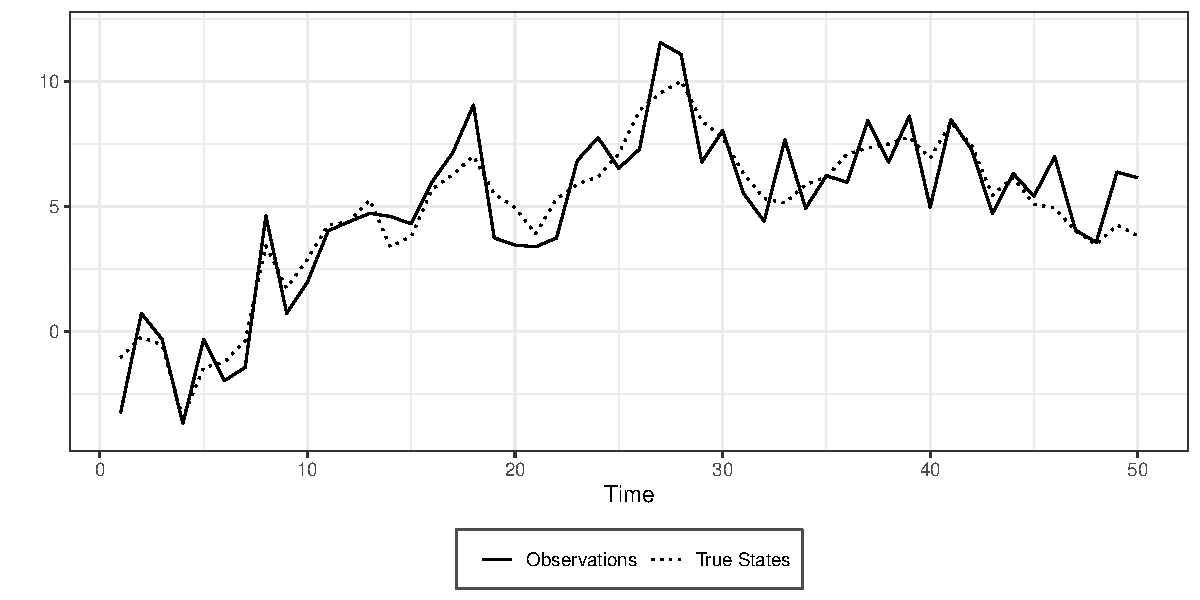
\includegraphics{new-draft_files/figure-latex/unnamed-chunk-5-1} 

}

\caption{Simulated random walk plus noise model}\label{fig:unnamed-chunk-5}
\end{figure}

The Kalman Filter for this model is implemented as described below.

\begin{algorithm} Kalman Filter for Random Walk plus Noise Model
\begin{itemize}
\item Initialize $\theta_{0} \sim N(m_{0},C_{0})$
\item For $t=1,...,n$:
\begin{enumerate}
\item Compute the one-step-ahead state predictive distribution at time $t-1$, notice that if $t=1$ no data have been observed yet and therefore $x_{1}|x_{0}\sim N(a_{1},R_{1})$ otherwise
\begin{align*}
x_{t}|y_{1:t-1} & \sim N(a_{t},R_{t})\\
a_{t} & = m_{t-1}\\
R_{t} & = C_{t-1}+\tau^2
\end{align*}
\item Compute the filtering distribution at time $t$ as $p(x_{t}|y_{1:t}) \propto p(x_{t}|y_{1:t-1})p(y_{t}|x_{t})$, i.e. the product of the one-step-ahead state predictive distribution and the likelihood
\begin{align*}
x_{t}|y_{1:t} & \sim N(m_{t},C_{t}) \\
m_{t} & = \big(1-\frac{R_{t}}{R_{t}+\sigma^2}\big)a_{t}+\frac{R_{t}}{R_{t}+\sigma^2}y_{t} \\
C_{t} & = \frac{R_{t}}{R_{t}+\sigma^2}\sigma^2
\end{align*}
\end{enumerate}
\end{itemize}
\end{algorithm}

Our \texttt{DLM} function implement in R replicate this steps.\\

\hrule
\hrule
\texttt{DLM(data,sig2,tau2,m0,C0)}
\hrule

\textbf{Arguments}

\texttt{data} ~~the observed process. It has to be a vector or a
univariate time series.\\
\texttt{sig2} ~~the variance \(\sigma^{2}\) in Equation (1)\\
\texttt{tau2} ~~the variance \(\tau^{2}\) in Equation (2)\\
\texttt{m0} ~~central value of the normal prior state distribution\\
\texttt{C0} ~~variance of the normal prior state distribution

\hrule
\hrule

\begin{Shaded}
\begin{Highlighting}[]
\NormalTok{DLM}\OtherTok{\textless{}{-}}\ControlFlowTok{function}\NormalTok{(data,sig2,tau2,m0,C0)\{}
\NormalTok{  n  }\OtherTok{=} \FunctionTok{length}\NormalTok{(data)}
\NormalTok{  m  }\OtherTok{=} \FunctionTok{rep}\NormalTok{(}\DecValTok{0}\NormalTok{,n)}
\NormalTok{  C  }\OtherTok{=} \FunctionTok{rep}\NormalTok{(}\DecValTok{0}\NormalTok{,n)}
  \ControlFlowTok{for}\NormalTok{ (t }\ControlFlowTok{in} \DecValTok{1}\SpecialCharTok{:}\NormalTok{n)\{}
    \ControlFlowTok{if}\NormalTok{ (t}\SpecialCharTok{==}\DecValTok{1}\NormalTok{)\{}
\NormalTok{      a }\OtherTok{=}\NormalTok{ m0}
\NormalTok{      R }\OtherTok{=}\NormalTok{ C0 }\SpecialCharTok{+}\NormalTok{ tau2}
\NormalTok{    \}}\ControlFlowTok{else}\NormalTok{\{}
\NormalTok{      a }\OtherTok{=}\NormalTok{ m[t}\DecValTok{{-}1}\NormalTok{]}
\NormalTok{      R }\OtherTok{=}\NormalTok{ C[t}\DecValTok{{-}1}\NormalTok{] }\SpecialCharTok{+}\NormalTok{ tau2}
\NormalTok{    \}}
\NormalTok{    A }\OtherTok{=}\NormalTok{ R}\SpecialCharTok{/}\NormalTok{(R}\SpecialCharTok{+}\NormalTok{sig2)}
\NormalTok{    m[t] }\OtherTok{=}\NormalTok{ (}\DecValTok{1}\SpecialCharTok{{-}}\NormalTok{A)}\SpecialCharTok{*}\NormalTok{a }\SpecialCharTok{+}\NormalTok{ A}\SpecialCharTok{*}\NormalTok{y[t]}
\NormalTok{    C[t] }\OtherTok{=}\NormalTok{ A}\SpecialCharTok{*}\NormalTok{sig2}
\NormalTok{  \}}
  \FunctionTok{return}\NormalTok{(}\FunctionTok{list}\NormalTok{(}\AttributeTok{m=}\NormalTok{m,}\AttributeTok{C=}\NormalTok{C))}
\NormalTok{\}}
\end{Highlighting}
\end{Shaded}

In Figure XX below filtered states estimated using Kalman Filter with
\(x_{0} \sim N(0,100)\) and \(\sigma^{2}=\tau^{2}=1\) are compared to
the true states values. Notice how closely the filtered states follow
the observations and the goodness of the approximation of the true
states. 95 percent credible intervals are computed as
\[[E(\theta_{t}|y_{1:t})-z_{1-\alpha/2}\sqrt{V(\theta_{t}|y_{1:t})},E(\theta_{t}|y_{1:t})+z_{1-\alpha/2}\sqrt{V(\theta_{t}|y_{1:t})}]\]

\begin{figure}[H]

{\centering 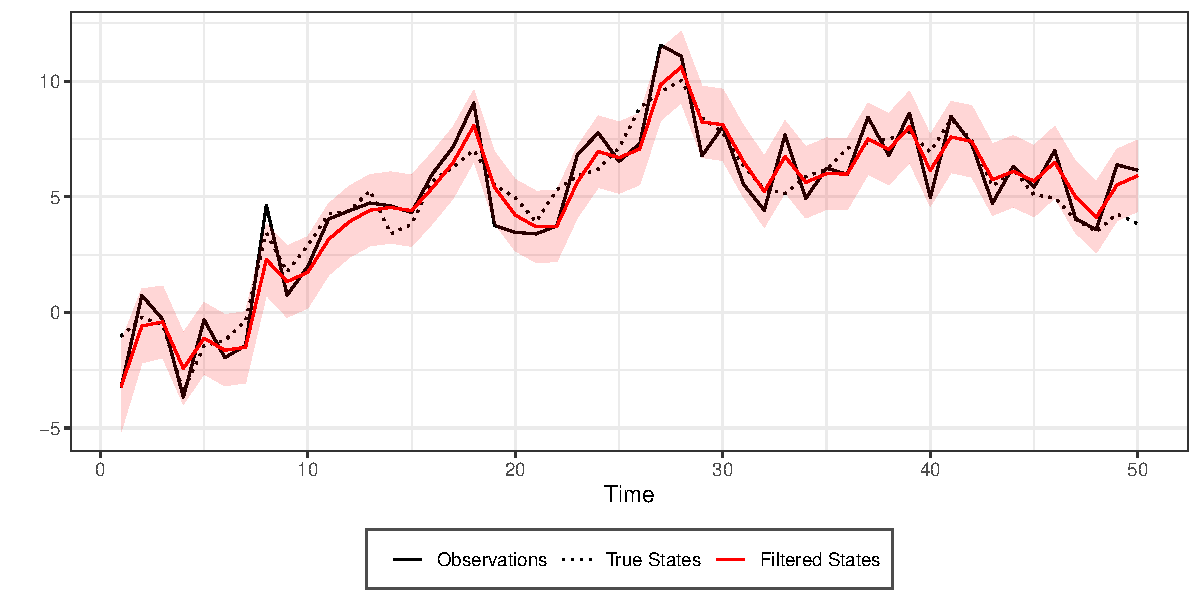
\includegraphics{new-draft_files/figure-latex/unnamed-chunk-7-1} 

}

\caption{Kalman Filtered States with credible interval (in red)}\label{fig:unnamed-chunk-7}
\end{figure}

The discussion of Kalman Filter will continue in Section XX where we
compare it to the Particle Filter.

\chapter{Particle Filter}

In the previous chapter we explained how the Kalman Filter is applied to
the case of a linear model with Gaussian errors to find closed-form
solution for the filtering and the predictive distributions.
Nonetheless, the majority of time-series models have a non-linear
structure and errors might follow non-Gaussian distributions.\\
In this chapter we describe \textit{particle filter} as an algorithm
that allows to update sequentially the filtering and the predictive
distributions in the non-linear and non-Gaussian case. Additionally, the
Kalman Filter can be seen as a special case of the more general particle
filter.\\
In section \ref{pf_intro} we introduce the fundamental notions of
\textit{importance sampling}, \textit{sequential importance sampling}
and \textit{resampling}. Then, in section \ref{pf_main} we describe
three particle filtering algorithms: the \textit{bootstrap}, the
\textit{guided} and the \{auxiliary particle filters\}. Instead, in
section \ref{pf_lui_west} we describe the \{Liu and West filter\}, when
particle filtering is used to estimate model's parameters. Finally, in
section \ref{pf_converg} we establish some general convergence results
for Particle Filter - Monte Carlo estimators.

\section{Introductory notions: sampling and resampling}\label{pf_intro}

Let \(\varphi: \mathcal X\rightarrow \mathbb R\) be a measurable,
integrable and bounded real-valued function, where
\((\mathcal X,\mathcal B(\mathcal X),\mathbb Q)\) is a probability
space.\footnote{$\mathcal B(\mathcal X)$ is the Borel sigma-algebra of $\mathcal X$.}
Suppose that the probability measure \(\mathbb Q\) admits a density
\(q(x)\) with respect to some measure \(\nu(dx)\) and it is feasible to
sample from that density.\\
To estimate the expected value of \(\varphi\) with respect to the
density \(q\), the basic Monte Carlo (MC) method would require to sample
\(N\) times from the target density \(q\) and to compute the average of
the function \(\varphi\) values. \(\hat \varphi_{MC}\) is the standard
MC estimator: \begin{equation*}
   \hat \varphi_{MC}=\frac{1}{N} \sum_{n=1}^N\varphi (X^n)\approx \mathbb E_q(\varphi)~~~X^n\thicksim q(\cdot)
\end{equation*} However, in many circumstances either it is impossible
to sample from the target density or there exist another density - call
it \(m(\cdot)\) - different from \(q\) that produces
\texttt{more\ efficient"\ estimates.\ \ In\ all\ the\ cases\ for\ which\ sampling\ takes\ place\ from\ a\ distribution\ different\ from\ the}correct"
(i.e., the true) one, importance sampling and resampling methods can be
applied (as augmented versions of the standard MC algorithm).

\subsection{Importance sampling}

Let us consider two probability spaces:
\((\mathcal X,\mathcal B(\mathcal X),\mathbb Q)\) and
\((\mathcal X,\mathcal B(\mathcal X),\mathbb M)\) and let the measurable
function \(w:\mathcal X\rightarrow \mathbb R\) be proportional to the
Radom-Nikodym derivative between \(\mathbb Q\) and \(\mathbb M\), i.e.,
\(w(x)\propto\frac{\mathbb Q(dx)}{\mathbb M(dx)}\).\\
The following result represents the starting point for the idea of
importance sampling.

\begin{lemma}\label{lemma_imp_sam_1}
For any measurable, integrable and bounded function $\varphi: \mathcal X\rightarrow \mathbb R$, the following holds:
\begin{equation}
    \mathbb E_\mathbb M(\varphi \cdot w)=\mathbb E_\mathbb Q(\varphi)\cdot \mathbb E_\mathbb M(w)
\end{equation}
\end{lemma}

\begin{proof*}
Note that $\mathbb Q(dx)=\frac{w(x)}{\mathbb E_\mathbb M(w)}\mathbb M(dx)$. Hence:
\begin{equation*}
    \mathbb E_\mathbb Q(\varphi)=\int_\mathcal X\varphi(x)\mathbb Q(dx)=\int_\mathcal X\varphi(x)\frac{w(x)}{\mathbb E_\mathbb M(w)}\mathbb M(dx)=\frac{\mathbb E_\mathbb M(\varphi \cdot w)}{\mathbb E_\mathbb M(w)}
\end{equation*}
$\hfill\blacksquare$
\end{proof*}

Lemma \ref{lemma_imp_sam_1} represents the key theoretical foundation of
\textbf{importance sampling} (IS), a numerical algorithm that allows to
sample from a \textit{proposal density} to estimate moments that are
computed with respect to the \textit{target density}, by means of
re-weighting the values of the target function \(\varphi\).\\
Adopting the previous notation, the target measure is \(\mathbb Q\),
while the proposal is \(\mathbb M\). IS requires to sample \(N\) values
from \(\mathbb M\), then to find the associated
\textit{normalized}\footnote{Weights are normalized when $\mathbb E_\mathbb M(W)=1$. In this case $W$ is the Radom-Nikodym derivative between $\mathbb Q$ and $\mathbb M$.}
weights \(W(X^n)\), finally to compute a weighted average of the values
taken by the function \(\varphi\). The IS is implemented according to
the following algorithm.

\begin{enumerate}
    \item Sample $N$ values from the proposal measure: $X^n\thicksim \mathbb M$ for $n=1,...,N$.
    \item Compute the associated normalized weights: $W(X^n)$ for $n=1,...,N$
    \item Compute the estimator:
    \begin{equation*}
        \hat \varphi= \frac{1}{N} \sum_{n=1}^N\varphi (X^n)W(X^n).
    \end{equation*}
\end{enumerate}

Note that \(\hat \varphi\) is an unbiased estimator for the target of
inference \(\mathbb E_\mathbb Q(\varphi)\). In fact: \begin{equation*}
    \begin{split}
        \mathbb E_\mathbb M(\hat \varphi)=\frac{1}{N} \sum_{n=1}^N \mathbb E_\mathbb M(\varphi \cdot W)=\mathbb E_\mathbb M(\varphi \cdot W)=\mathbb E_\mathbb Q(\varphi)
    \end{split}
\end{equation*} where the last equality follows from lemma
\ref{lemma_imp_sam_1} and the fact that weights are normalized to 1.

\subsubsection{Auto-normalized IS}

Usually, the Radom-Nikodym derivative is known up to a normalizing
constant and the IS algorithm has to be described in more general terms.
In the previous section the \textit{normalized} weighting function
\(W(\cdot)\) was the Radom-Nikodym derivative of \(\mathbb Q\) with
respect to \(\mathbb M\). More generally, consider the function
\(w(x)\propto\frac{\mathbb Q(dx)}{\mathbb M(dx)}\), denoted as
\textit{importance function}, proportional to the derivative
\(W(\cdot)\).\\
In this case, weights have to be \textit{auto}-normalized to obtain the
IS - Monte Carlo estimator. The auto-normalized IS is implemented
according to the following procedure.

\begin{enumerate}
    \item Sample $N$ values from the proposal measure: $X^n\thicksim \mathbb M$ for $n=1,...,N$.
    \item Compute the associated \textit{un-normalized} weights: $w(X^n)$ for $n=1,...,N$.
    \item Normalize the weights, for $n=1,...,N$:
    \begin{equation*}
        W^n:=\frac{w(X^n)}{\sum_{m=1}^Nw(X^m)}
    \end{equation*}
    \item Compute the estimator:
    \begin{equation*}
        \hat \varphi_{AN}=\sum_{n=1}^N\varphi (X^n)W^n
    \end{equation*}
\end{enumerate}

While the auto-normalized estimator is biased (since \(W^n\) involves a
ratio of random variables), it is consistent (see \ref{pf_is_conv} for
details). ~\\
It is useful to interpret IS as an algorithm that allows to find an
approximation for the probability measure \(\mathbb Q\) as a weighted
average of Dirac measures for the sampled values (\(X^n\)):
\(\delta_{X^n}(dx)\) where the weights are the auto-normalized ones
(\(W^n\)). In particular: \begin{equation}
    \mathbb Q^N(dx):=\sum_{n=1}^NW^n\delta_{X^n}(dx), ~~~X^n\thicksim \mathbb M
\end{equation} Furthermore, the IS estimator is the expected value of
the function \(\varphi\) with respect to the approximating probability
measure \(\mathbb Q^N\): \begin{equation*}
    \begin{split}
        \mathbb E_{\mathbb Q^N}(\varphi)=&\int_\mathcal X\varphi(x)\mathbb Q^N(dx)=\int_\mathcal X\varphi(x)\sum_{n=1}^NW^n\delta_{X^n}(dx)=\\
       = &\sum_{n=1}^N\int_\mathcal X\varphi(x)W^n\delta_{X^n}(dx)=\sum_{n=1}^N\varphi (X^n)W^n=\hat \varphi_{AN}
    \end{split}
\end{equation*}

\subsubsection{Convergence of the IS estimator}\label{pf_is_conv}

Consider the auto-normalized IS estimator
\(\hat \varphi= \sum_{n=1}^N\varphi (X^n)W^n\). We can write:
\begin{equation*}
   \hat \varphi_{AN} - \mathbb E_{\mathbb Q}(\varphi)=\mathbb E_{\mathbb Q^N}(\varphi)-\mathbb E_{\mathbb Q}(\varphi)=\frac{N^{-1}\sum_{n=1}^Nw(X^n)[\varphi(X^n)-\mathbb E_{\mathbb Q}(\varphi)]}{N^{-1}\sum_{n=1}^Nw(X^n)}
\end{equation*} Let
\(\bar \varphi(X):=\varphi(X)-\mathbb E_{\mathbb Q}(\varphi)\). Applying
the CLT to the numerator, assuming that
\(\mathbb E_{\mathbb M}(w^2\bar\varphi^2)<+\infty\), we get:
\begin{equation}
    \sqrt{N}\Bigg\{\frac{1}{N}\sum_{n=1}^Nw(X^n)\bar \varphi (X^n)\Bigg\}\implies \mathcal N\big(0,\mathbb E_{\mathbb M}(w^2\bar\varphi^2)\big)\label{is_conv_clt}
\end{equation} where \(\implies\) denotes convergence in distribution.
Instead, for the denominator the strong LLN implies that:
\begin{equation}
    \frac{1}{N}\sum_{n=1}^Nw(X^n)\rightarrow \mathbb E_{\mathbb M}(w) ~~~\text{ a.s.}\label{is_conv_lln}
\end{equation} Applying Slutsky's theorem, together with
\eqref{is_conv_clt} and \eqref{is_conv_lln}, we obtain: \begin{equation}
   \sqrt{N}\big[  \hat \varphi_{AN} - \mathbb E_{\mathbb Q}(\varphi)\big] \implies \mathcal N\Bigg(0,\frac{\mathbb E_{\mathbb M}(w^2\bar\varphi^2)}{[\mathbb E_{\mathbb M}(w)]^2}\Bigg)
\end{equation} Therefore, the IS (auto-normalized) estimator for
\(\varphi\) is both consistent and asymptotically normal.

\subsubsection{Effective Sample Size}

A common measure of efficiency for IS is the
\textit{effective sample size} (ESS), defined as: \begin{equation*}
    ESS(W^{1:N}):=\frac{1}{\sum_{n=1}^N(W^n)^2}=\frac{[\sum_{n=1}^N w(X^n)]^2}{\sum_{n=1}^N(w(X^n))^2}
\end{equation*} Observe that the \(ESS\) lies in the interval \([1,N]\).
For instance, if \(W^n=1/N\), as in the case of the standard MC method,
\(ESS=N\).\\
It is possible to relate the \(ESS\) to the variance of the importance
function. In fact: \begin{equation*}
    \frac{N}{ESS}=1+\frac{N^{-1}\sum_{n=1}^N(w(X^n))^2-\big[N^{-1}\sum_{n=1}^N w(X^n)\big]^2}{\big[N^{-1}\sum_{n=1}^N w(X^n)\big]^2}
\end{equation*} The second term in the numerator of the previous formula
is the square of the coefficient of variation (i.e., the ratio between
the variance and the squared mean) of the un-normalized weights. It is
clear that a lower \(ESS\) is associated with a higher variance for the
weights.

\subsection{Sequential Importance Sampling}

When dealing with state-space models, the importance sampling algorithm
has to be applied dynamically and the importance weights are updated
period-by-period. To illustrate the relevance of the
\textit{sequential importance sampling} (SIS) algorithm, we consider a
two-period stochastic process.~\\
Let us consider the approximation of the measure \(\mathbb Q_0\)
obtained at time 0 through IS from the measure \(\mathbb M_0\):
\begin{equation*}
    \mathbb Q_0^N(dx_0)=\sum_{n=1}^NW_0^n\delta_{X_0^n}(dx_0),~~\text{with } X_0^n\thicksim \mathbb M_0,~~\text{and }  W_0^n:=\frac{w_0(X_0^n)}{\sum_{m=1}^Nw_0(X_0^m)}.
\end{equation*} Moreover, let \(M_1(x_0,dx_1)\) be the transition
kernel. We want to update, sequentially, the approximating measure
\(\mathbb Q_0\) to obtain an approximation of the measure:
\begin{equation*}
    \mathbb Q_{1}(dx_{0:1})=\mathbb Q_0(dx_0)M_1(x_0,dx_1)
\end{equation*} SIS works according to the following algorithm.

\begin{enumerate}
    \item Sample $N$ values for $X_0$ from the proposal measure $\mathbb M_0$: $X_0^n\thicksim \mathbb M_0$ for $n=1,...,N$.
    \item Sample $N$ values for $X_1$ from the transition kernel $M_1$: $X_1^n\thicksim M_1(X_0^n,dx_1)$ for $n=1,...,N$.
    \item Compute the auto-normalized weights. In this case, they are computed taking into account only time 0 sampled observations since $X_1^n$ is sampled from the correct distribution: $W_1^n=W_0^n$.
\end{enumerate}

Therefore, the particle approximation of \(\mathbb Q_{1}(dx_{0:1})\) is:
\begin{equation*}
      \mathbb Q_{1}^N(dx_{0:1})=\sum_{n=1}^NW_0^n\delta_{X_0^n}(dx_0)M_1(X_0^n,dx_1)
\end{equation*}

\subsection{Sequential Importance Resampling}

A second approach can be used when sampling has to be done sequentially:
\textit{sequential importance resampling} (SIR). Differently from SIS,
an intermediate resampling stage takes place, in which time 0 values are
sampled with replacement according to a given resampling strategy
(usually, sampling indexes from a multinomial distribution with
probabilities equal to the weights computed through IS at time 0).\\
While in the SIS all the particles (i.e., the sampled values)
\texttt{survive",\ with\ the}risk" that particles associated with small
weights are carried-over (in the sense that sampling in period 1 occurs
from the kernel \(M_1(X_0^n,dx_1)\)), the same does not occur in SIR. In
this second algorithm, particles with larger weights are more likely to
be resampled and be used to ``generate" the particles in the next
period.\\
We describe the SIR more formally, focusing on the previous two-period
case.

\begin{enumerate}
    \item Sample $N$ values $X_0$ from the proposal measure $\mathbb M_0$: $X_0^n\thicksim \mathbb M_0$ for $n=1,...,N$.
    \item Compute the weights $W_0^n$ for $n=1,...,N$.
    \item Sample $N$ indexes $(A_1^1,...A_1^N)$ from a multinomial distribution such that for all $j=1,...N$, $Pr(\{A_1^j=n\})=W_0^n$, for all $n=1,...N$.
    \item Build a new time 0 sample, using the values for $X_0$ associated to the previously extracted indexes $(A_1^n)_{n}$: $(X_0^{A_1^1},...,X_0^{A_1^N})$.
    \item Sample $N$ values for $X_1$ from the transition kernel $M_1$: $X_1^n\thicksim M_1(X_0^{A_1^n},dx_1)$ for $n=1,...,N$.
\end{enumerate}

Steps 3-4 constitute the actual resampling ones. At this point, let us
define the new two-period sequence
\(\tilde X_{0:1}^n:=(X_0^{A_1^n},X_1^n)\). Then, the particle
approximation for the joint distribution of \((X_0,X_1)\) becomes:
\begin{equation*}
     \mathbb Q_{1}^N(dx_{0:1})=\frac{1}{N}\sum_{n=1}^N\delta_{\tilde X_{0:1}^n}(dx_{0:1})
\end{equation*} Note that, after resampling occurred, each particle
\(\tilde X_{0:1}^n:=(X_0^{A_1^n},X_1^n)\) has the same probability
weight.\\
To understand the reason of the previous statement, let us assume that
both \(\mathbb Q_0\) and \(\mathbb M_0\) admit densities \(q_0\),
\(m_0\) with respect to the same dominating measure \(\nu(dx_0)\) and
that the transition kernel \(M_1\) also admits the density \(m_1\).
Consider the sequential updating for the weights: \begin{equation}
    w^n_1=\frac{\mathbb Q_1(\tilde dx_{0:1})}{\mathbb M_1(dx_{0:1})}\propto \frac{q_0(x_0^{A_1^n})}{Pr(A_1^n)\cdot m_0(x_0^{A_1^n})}\cdot \frac{m_1(x_1^n|x_0^{A_1^n})}{m_1(x_1^n|x_0^{A_1^n})}
=\underbrace{\frac{q_0(x_0^{A_1^n})}{ m_0(x_0^{A_1^n})}}_{W_0^n}\cdot \underbrace{\frac{1}{Pr(A_1^n)}}_{1/W_0^n}=1\label{sis_update}
\end{equation} where \(\mathbb M_1\) denotes the probability measure for
the extraction of the particle \(\tilde x_{0:1}^n\) according to SIR.
\(\mathbb M_1\) (second equality sign in the previous formula) can be
rewritten as the product between the kernel for \(x_1^n\) given
\(x_0^{A_1^n}\) and the probability of \(x_0^{A_1^n}\) itself. This last
probability can also be rewritten as the product between the proposal
density \(m_0\) from which \(X_0\) is extracted and the probability that
it is sampled again when resampling occurs.

\subsection{SIS vs SIR}

The choice between the two sequential sampling strategies (SIS and SIR)
has significant implications in terms of computational cost and variance
of the importance weights. In fact, it is clear that SIR is more costly
computationally since it requires an intermediate resampling step.
Nonetheless, SIS suffers from the problem knonw as
\textit{curse of dimensionality}, i.e., the fact that the \(ESS\)
collapses over time as the variance of the weights diverges.\\
Consider an extension of SIS to a \(T\)-period model and let us assume
that the target and the proposal kernels admit densities, respectively,
\(q_t\) and \(m_t\) with respect to the same dominating measures (this
implies that the joint
distributions\footnote{Let us denote the joint distributions with $q_t$ and $m_t$ too, with some abuse of notation}
admit a density too). Then, weights, for every \(t=1,...,T\), are
updated according to: \begin{equation}
    w_t^n\propto \frac{q_t(x_{0:t}^n)}{m_t(x_{0:t}^n)}\propto \underbrace{\frac{q_{t-1}( x_{0:t-1}^n)}{m_{t-1}(x_{0:t-1}^n)}}_{\propto w_{t-1}^n}\cdot \frac{q_t( x_t|x_{t-1}^n)}{m_t(x_t|x_{t-1}^n)}\propto 
    w_{t-1}^n\cdot\frac{q_t( x_t|x_{t-1}^n)}{m_t(x_t|x_{t-1}^n)}\label{sis_update}
\end{equation} Equation \eqref{sis_update} suggests, intuitively, that
over time new variance is added from the incremental weights (i.e., the
updating factor \(q_t( x_t|x_{t-1}^n)/m_t( x_t|x_{t-1}^n)\)) determining
the curse of dimensionality issue. Instead, when resampling takes place,
since the past weights \(w_{t-1}\) are reset to be equal across them all
the variance of \(w_t\) inherited from the past is shut-down and the
only source of variability at each stage comes from the incremental
weights.

\section{Particle Filter}\label{pf_main}

\color{red}

Let us consider the standard state-space model introduced in the
previous chapters. \color{black} \textit{Particle filter} (PF) is a
numerical algorithm that is used to obtain approximations for the
filtering - \(\mathbb P_t (dx_t|y_{1:t})\) - and the prediction -
\(\mathbb P_t (dx_t|y_{1:t-1})\) - distributions for inference in
state-space models.~\\
In a state-space model sampling sequentially from the transition kernels
for the states is not enough to obtain good approximations since the
observation sample (\(y_{1:T}\)) contains information about the
underlying states through the likelihood function \(f_t(y_t|x_t)\).
Observations constitute signals for the model's states.\\
Therefore, the conditional distribution of the states, given the
observed data - \(\mathbb P_t(dx_{1:t}|y_{1:t})\) - changes over time as
new data points become available. The PF algorithm allows to incorporate
sequentially the new data to obtain new approximations for this
distribution (and for the filtering and prediction ones).\\
In general, at each step of the algorithm, states are sampled
sequentially from the proposal measure, call it \(\mathbb M_t\), and
importance auto-normalized weights are computed as the Radom-Nikodym
derivative of the target \(\mathbb P_t\) with respect to the proposal
\(\mathbb M_t\). Moreover, the Markov properties of the sequence of the
states allows to update sequentially the importance weights.~\\
We will analyse three different types of particle filtering procedures:
\textit{bootstrap}, \textit{guided} and
\textit{auxiliary particle filters}, that differ between them with
respect to their scope and efficiency.

\subsection{Degeneracy of the SIS in Particle Filter}

Usually, PF requires a resampling step at each stage of the algorithm.
Recall that, in general, resampling determines a trade-off between the
increase in the variance at the resampling stage and a decrease in the
variance when future states are sampled from the transition kernel.\\
\texttt{Dead"\ particles\ (i.e.,\ those\ with\ small\ weights)\ are\ \ likely\ to\ be\ removed\ when\ resampling\ takes\ place\ and\ past\ weights\ get}reset"
(usually, they are set to be equal to \(1/N\)). Otherwise, the
\textit{curse of dimensionality} problem will emerge and the variance of
the weights will diverge over time as the variance of past weights
increases as new updates occur period-by-period. Figure ***** shows an
example of a PF where SIS is used: note that the \(ESS\) drops
dramatically after few periods, meaning that the variance of the
importance weights diverges. This motivates the use of a SIR structure
for the PF algorithm.~\\
Lastly, it is now common practice to use a mixed approach with respect
to resampling (recall that resampling has an additional computational
cost). Generally, resampling is done \textit{adaptively}, when some
condition is met. A standard criterion that is used (and that we adopt
in our implementations of the PF) is to resample when the \(ESS\) drops
below some threshold \(ESS_{min}\in [1,N]\): \begin{equation}
    ESS(W_{t-1}^{1:N})<ESS_{min}
\end{equation}

\section{Implementation}

Consider again the random walk plus noise model of section XX,the
challenge here is to estimate the filtered states using a Sequential
Importance Sampling algorithm. The main idea of the SIS applied to this
univariate linear gaussian model is described in the following
algorithm. We indicate with \(n\) the sample size of time observations
and with \(N\) the generated sample size for each step of the Sequenial
Monte Carlo.

\begin{algorithm} SIS filter for Random Walk plus Noise Model
\begin{itemize}
\item Let $\{(x_{0},w_{0})^{(i)}\}_{i=1}^{N}$ summarizes $p(x_{0}|y_{0})$ such that, for example, $E(g(x_{0})|y_{0}) \approx \sum_{i=1}^{N}w_{0}^{(i)}g(x_{0}^{(i)})$. In particular, initialize $(x_{0}^{(1)},...,x_{0}^{(N)})$ form $N(m_{0},C_{0})$ and set $w_{0}^{(i)}=N^{-1} \ \forall \ i=1,...,N$.
\item For $t=1,...,n$:
\begin{enumerate}
\item Draw $x_{t}^{(i)} \sim N(x_{t-1}^{(i)},\tau^2) \ \ i=1,...,N$ such that $\{(x_{t},w_{t-1})^{(i)}\}_{i=1}^{N}$ summarizes $p(x_{t}|y_{t-1})$
\item Set $w_{t}^{(i)} = w_{t-1}^{(i)}f_{N}(y_{t};x_{t}^{(i)},\sigma^2) \ \ i=1,...,N$ such that $\{(x_{t},w_{t})^{(i)}\}_{i=1}^{N}$ summarizes $p(x_{t}|y_{t})$
\item Set $p(x_{t}|y_{t})=\sum_{i=1}^{N}w_{t}^{(i)}\delta_{x_{t}^{(i)}}$
\end{enumerate}
\end{itemize}
\end{algorithm}

Our \texttt{SISfun} function implemented in R replicate this steps.\\

\hrule
\hrule
\texttt{SISfun(data,N,m0,C0,tau,sigma)}
\hrule

\textbf{Arguments}

\texttt{data} ~~the observed process. It has to be a vector or a
univariate time series.\\
\texttt{N} ~~number of particles generated at each step\\
\texttt{m0} ~~central value of the normal prior state distribution\\
\texttt{C0} ~~variance of the normal prior state distribution\\
\texttt{tau} ~~the standard deviation \(\tau\) in Equation (2)\\
\texttt{sigma} ~~the standard deviation \(\sigma\) in Equation (1)

\hrule
\hrule

\begin{Shaded}
\begin{Highlighting}[]
\NormalTok{SISfun}\OtherTok{\textless{}{-}}\ControlFlowTok{function}\NormalTok{(data,N,m0,C0,tau,sigma)\{}
\NormalTok{  xs}\OtherTok{\textless{}{-}}\ConstantTok{NULL}
\NormalTok{  ws}\OtherTok{\textless{}{-}}\ConstantTok{NULL}
\NormalTok{  ess}\OtherTok{\textless{}{-}}\ConstantTok{NULL}
\NormalTok{  x  }\OtherTok{=} \FunctionTok{rnorm}\NormalTok{(N,m0,}\FunctionTok{sqrt}\NormalTok{(C0))}
\NormalTok{  w  }\OtherTok{=} \FunctionTok{rep}\NormalTok{(}\DecValTok{1}\SpecialCharTok{/}\NormalTok{N,N)}
  \ControlFlowTok{for}\NormalTok{(t }\ControlFlowTok{in} \DecValTok{1}\SpecialCharTok{:}\FunctionTok{length}\NormalTok{(data))\{}
\NormalTok{    x    }\OtherTok{=} \FunctionTok{rnorm}\NormalTok{(N,x,tau)                   }\CommentTok{\#sample from N(x\_\{t{-}1\},tau)}
\NormalTok{    w    }\OtherTok{=}\NormalTok{ w}\SpecialCharTok{*}\FunctionTok{dnorm}\NormalTok{(data[t],x,sigma)         }\CommentTok{\#update weight}
\NormalTok{    xs }\OtherTok{=} \FunctionTok{rbind}\NormalTok{(xs,x)}
\NormalTok{    ws }\OtherTok{=} \FunctionTok{rbind}\NormalTok{(ws,w)}
    
\NormalTok{    wnorm}\OtherTok{=}\NormalTok{ w}\SpecialCharTok{/}\FunctionTok{sum}\NormalTok{(w)                         }\CommentTok{\#normalized weight}
\NormalTok{    ESS  }\OtherTok{=} \DecValTok{1}\SpecialCharTok{/}\FunctionTok{sum}\NormalTok{(wnorm}\SpecialCharTok{\^{}}\DecValTok{2}\NormalTok{)                   }\CommentTok{\#effective sample size}
    
\NormalTok{    ess }\OtherTok{=}\FunctionTok{rbind}\NormalTok{(ess,ESS)}
\NormalTok{  \}}
  
  \FunctionTok{return}\NormalTok{(}\FunctionTok{list}\NormalTok{(}\AttributeTok{xs=}\NormalTok{xs,}\AttributeTok{ws=}\NormalTok{ws,}\AttributeTok{ess=}\NormalTok{ess))}
\NormalTok{\}}
\end{Highlighting}
\end{Shaded}

We have already discussed the reasons why the SIS algorithm does not
provide a good strategy in the filtering problem. We provide a graphical
intuition of what happens when we use such filtering strategy on a
simulated dataset. We decide to set \(N=1000\),\(m_{0}=0\),\(C_{0}=100\)
and \(\tau=\sigma=1\). The results shown in the following two plots
shows a clear degeneration of the effective sample size and bad fit of
filtered states with respect to the true values.

\begin{figure}[H]

{\centering 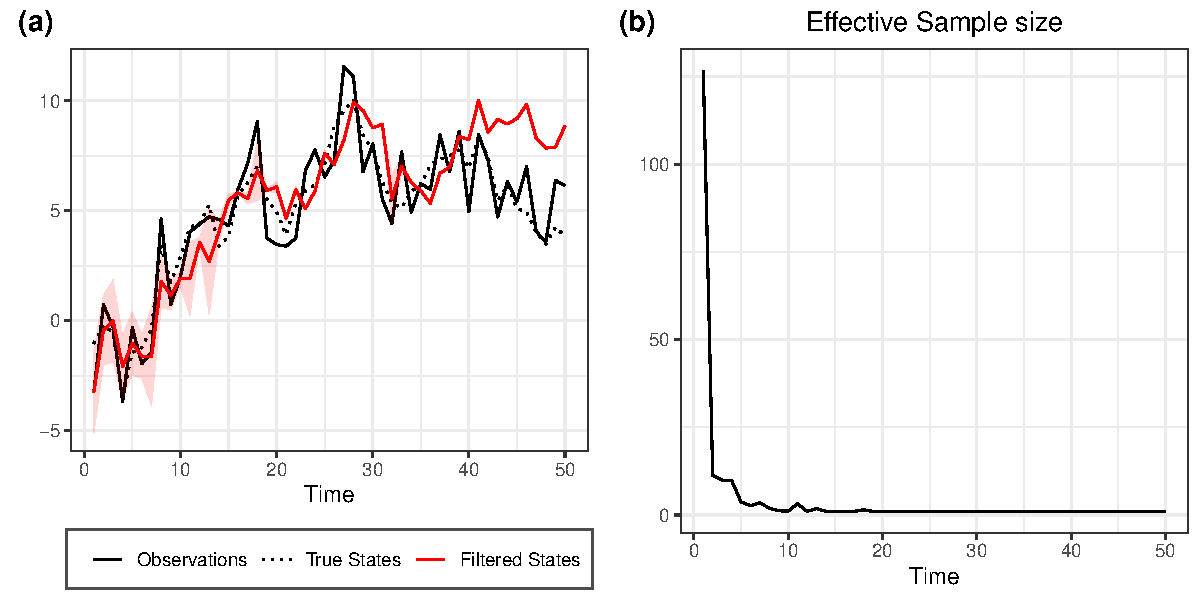
\includegraphics{new-draft_files/figure-latex/unnamed-chunk-10-1} 

}

\caption{a) SIS Filtered States with credible interval (in red). b) Effective sample size.}\label{fig:unnamed-chunk-10}
\end{figure}

\subsection{Bootstrap Particle Filter}

The bootstrap particle filter (BPF) is the easiest form of an adaptive
PF algorithm. In fact, future states are sampled from the
\textit{correct} transition kernel and the weights are updated
sequentially using the likelihood \(f_t(y_t|x_t)\).\\
We summarize the procedure with the following scheme.

\begin{enumerate}
    \item \textbf{Inital stage: }For $n=1,...,N$, at time 0 sample: $X_0^n\thicksim\mathbb P_0(dx_0)$ and set the un-normalized weights $w_0^n=1$.\
    Then, the normalized weights are: $W_0^n=\frac{1}{N}$.
    \item \textbf{For every $t=1,...T$:}
    \begin{enumerate}
        \item \textbf{Resample} if $ESS(W_{t-1}^{1:N})<ESS_{min}$:\footnote{It is indifferent to implement this resampling step at the beginning or at the end of each iteration (as we do in our codes) as long as the initial stage $t=0$ generates weights that are constant and equal to $1/N$. In fact, in this case, resampling will never take place at the beginning of the first iteration since $ESS(W_0^n=1/N)=N$ that is larger than or equal to $ESS_{min}$.\
        However, when we describe the algorithm, we chose to leave this resampling step at the beginning of each iteration. In fact, when considering the guided or auxiliary PF, we can, more generally, sample the initial values (time $t=0$) for the state from a proposal distribution different from the target one. In this case, the weights at $t=0$ might differ from $1/N$, hence resampling might take place already at the beginning of the first iteration.}
\begin{enumerate}
    \item Multinomial sampling for the indexes $(A_t^n)_n$ with probabilities given by $(W_{t-1}^n)_{n}$.
    \item Update weights as: $\hat w_{t-1}^n = 1$ for $n=1,...,N$.
\end{enumerate}
\textbf{Otherwise, } 
\begin{enumerate}
    \item Set the indexes: $A_t^{n}=n$ for $n=1,...,N$.
    \item Set the weights: $\hat w_{t-1}^n = w_{t-1}^n$ for $n=1,...,N$.
\end{enumerate}
\item Sample the future states from the transition kernel: $X_t^n\thicksim P_t(X_{t-1}^{A_t^n},dx_t)$  for $n=1,...,N$.
\item Update the un-normalized weights through the likelihood function for $n=1,...,N$.:
\begin{equation*}
    w_t^n=\hat w_{t-1}^n\cdot f_t(y_t|X_t^n).
\end{equation*}
\item Normalize the weights  for $n=1,...,N$.: $W_t^n:=\frac{w_t^n}{\sum_{m=1}^Nw_t^m}$.
    \end{enumerate}
\end{enumerate}

Therefore, at the initial step the pre-sample period states \(x_0^n\)
are extracted and every sampled state is assigned an equal weight since
there is no corresponding observation \(y_0\) that gives additional
information on the likelihood of that extraction.\\
Resampling does never take place in
\(t=1\)\footnote{Since $ESS(W_0^n=1/N)=N\geq ESS_{min}$.} and the state
in \(t=1\) is sampled from the correct transition kernel
\(P_1(x_0^n,dx_1)\). Now, the time 0 weights are updated incorporating
the information from the data point \(y_1\) in a very intuitive way:
more \textit{likely} states (given \(y_1\)) are given higher weights:
\(w_1^n=f_1(y_1|x_1^n)\). This weights are used to approximate the time
\(1\) filtering distribution.\\
At a subsequent stage, the \(ESS\) criterion should be checked and, in
case it is satisfied, resampling takes place and time \(1\) weights are
reset to be equal to \(1/N\).~\\
The key characteristic of the PF is the fact that the importance weights
are updated sequentially, according to the ``information" provided by
the observed data (i.e., the sequence \(y_{1:T}\)). Recall that time
\(t\) weight is the Radom-Nikodym derivative of the target with respect
to the proposal distribution. In the BPF, the time \(t\) target is the
measure \(\mathbb P_t(dx_{0:t}|y_{1:t})\), while the proposal, denoted
generically by \(\mathbb M_t\), is
\(\mathbb M_t(dx_{0:t}|y_{1:t})=\mathbb M_{t-1}(dx_{0:t-1}|y_{1:t-1})\cdot P_t(x_{t-1},dx_t)\).
Hence: \begin{equation}
    \begin{split}
        w_t\propto&\frac{\mathbb P_t(dx_{0:t}|y_{1:t})}{\mathbb M_t(dx_{0:t}|y_{1:t})}\propto \frac{\mathbb P_{t-1}(dx_{0:t-1}|y_{1:t-1})\cdot P_t(x_{t-1},dx_t)\cdot f(y_t|x_t)}{\mathbb M_{t-1}(dx_{0:t-1}|y_{1:t-1})\cdot P_t(x_{t-1},dx_t)}=\\
        =&\underbrace{\frac{\mathbb P_{t-1}(dx_{0:t-1}|y_{1:t-1})}{\mathbb M_{t-1}(dx_{0:t-1}|y_{1:t-1})}}_{\hat w_{t-1}}\cdot f(y_t|x_t)=\hat w_{t-1}\cdot f(y_t|x_t)
    \end{split}\label{weight_updated_bpf}
\end{equation} Finally, the BPF is able to generate the two key objects
for inference in state-space models:

\begin{itemize}
    \item the predictive distribution:
    \begin{equation}
    \begin{split}
        \mathbb P_t^N (dx_t|y_{1:t-1})=&\frac{1}{\sum_{n=1}^N\hat w_t^n}\sum_{n=1}^N\hat w_t^n\delta_{X_t^n}(dx_t)=\\
        =&\begin{cases}
        \frac{1}{N}\sum_{n=1}^N\delta_{X_t^n}(dx_t)
        ~~~~~~~~~~~~~~~~ ~\text{ if resampling occurs}\\
        \frac{1}{\sum_{n=1}^N w_{t-1}^n}\sum_{n=1}^Nw_{t-1}^n\delta_{X_t^n}(dx_t)~~~~ \text{ otherwise}
        \end{cases},
        \end{split}
    \end{equation}
    \item the filtering distribution:
    \begin{equation}
        \mathbb P_t^N (dx_t|y_{1:t})=\sum_{n=1}^NW_t^n\delta_{X_t^n}(dx_t)
    \end{equation}
\end{itemize}

\section{Implementation}

In this section, Bootstrap Particle Filter will be used to estimate
filtered states of the Random Walk plus Noise introduced in section XX.
The overall strategy replicate the SIS filter with the addition of a
ESS-based resampling step that applies when the effective sample size is
smaller than a predetermined threshold opportunely chosen (in our
example we decide to follow a common rule of thumb consisting in setting
the threshold at \(N/2\)). The steps are presented in the following
algorithm.

\begin{algorithm} BPF for Random Walk plus Noise Model
\begin{itemize}
\item Let $\{(x_{0},w_{0})^{(i)}\}_{i=1}^{N}$ summarizes $p(x_{0}|y_{0})$ such that, for example, $E(g(x_{0})|y_{0}) \approx \sum_{i=1}^{N}w_{0}^{(i)}g(x_{0}^{(i)})$. In particular, initialize $(x_{0}^{(1)},...,x_{0}^{(N)})$ form $N(m_{0},C_{0})$ and set $w_{0}^{(i)}=N^{-1} \ \forall \ i=1,...,N$.
\item For $t=1,...,n$:
\begin{enumerate}
\item Draw $x_{t}^{(i)} \sim N(x_{t-1}^{(i)},\tau^2) \ \ i=1,...,N$ such that $\{(x_{t},w_{t-1})^{(i)}\}_{i=1}^{N}$ summarizes $p(x_{t}|y_{t-1})$
\item Set $w_{t}^{(i)} = w_{t-1}^{(i)}f_{N}(y_{t};x_{t}^{(i)},\sigma^2) \ \ i=1,...,N$ such that $\{(x_{t},w_{t})^{(i)}\}_{i=1}^{N}$ summarizes $p(x_{t}|y_{t})$
\item if $ESS<N/2$ then
\begin{enumerate}
\item Draw a sample of size N, $(x_{t}^{(1)},...,x_{t}^{(N)})$, from the discrete distribution $P(x_{t}=x_{t}^{(i)})=w_{t}^{(i)},\ \ i=1,...,N$
\item Reset the weights: $w_{t}^{(i)}=N^{-1}$, $i=1,...,N$.
\end{enumerate}
\item Set $p(x_{t}|y_{t})=\sum_{i=1}^{N}w_{t}^{(i)}\delta_{x_{t}^{(i)}}$
\end{enumerate}
\end{itemize}
\end{algorithm}

These steps are resumed in our \texttt{PFfun} function.\\

\hrule
\hrule
\texttt{PFfun(data,N,m0,C0,tau,sigma,r)}
\hrule

\textbf{Arguments}

\texttt{data} ~~the observed process. It has to be a vector or a
univariate time series.\\
\texttt{N} ~~number of particles generated at each step\\
\texttt{m0} ~~central value of the normal prior state distribution\\
\texttt{C0} ~~variance of the normal prior state distribution\\
\texttt{tau} ~~the standard deviation \(\tau\) in Equation (2)\\
\texttt{sigma} ~~the standard deviation \(\sigma\) in Equation (1)\\
\texttt{r} ~~ if present the threshold is set equal to \(N/r\)
otherwise, if missing, the threshold is set equal to \(N/2\)

\hrule
\hrule

\begin{Shaded}
\begin{Highlighting}[]
\NormalTok{PFfun}\OtherTok{\textless{}{-}}\ControlFlowTok{function}\NormalTok{(data,N,m0,C0,tau,sigma,r)\{}
  \ControlFlowTok{if}\NormalTok{(}\FunctionTok{missing}\NormalTok{(r))\{r}\OtherTok{=}\DecValTok{2}\NormalTok{\}}\ControlFlowTok{else}\NormalTok{\{\}}
\NormalTok{  xs}\OtherTok{\textless{}{-}}\ConstantTok{NULL}
\NormalTok{  ws}\OtherTok{\textless{}{-}}\ConstantTok{NULL}
\NormalTok{  ess}\OtherTok{\textless{}{-}}\ConstantTok{NULL}
\NormalTok{  x  }\OtherTok{=} \FunctionTok{rnorm}\NormalTok{(N,m0,}\FunctionTok{sqrt}\NormalTok{(C0))}
\NormalTok{  w  }\OtherTok{=} \FunctionTok{rep}\NormalTok{(}\DecValTok{1}\SpecialCharTok{/}\NormalTok{N,N)}
   
  \ControlFlowTok{for}\NormalTok{(t }\ControlFlowTok{in} \DecValTok{1}\SpecialCharTok{:}\FunctionTok{length}\NormalTok{(data))\{}
    
\NormalTok{    x}\OtherTok{\textless{}{-}}\FunctionTok{rnorm}\NormalTok{(N,x,tau)}
\NormalTok{    w1}\OtherTok{\textless{}{-}}\NormalTok{w}\SpecialCharTok{*}\FunctionTok{dnorm}\NormalTok{(data[t],x,sigma)}
    
\NormalTok{    w }\OtherTok{=}\NormalTok{ w1}\SpecialCharTok{/}\FunctionTok{sum}\NormalTok{(w1)}
\NormalTok{    ESS  }\OtherTok{=} \DecValTok{1}\SpecialCharTok{/}\FunctionTok{sum}\NormalTok{(w}\SpecialCharTok{\^{}}\DecValTok{2}\NormalTok{)}
    
    \ControlFlowTok{if}\NormalTok{(ESS}\SpecialCharTok{\textless{}}\NormalTok{(N}\SpecialCharTok{/}\NormalTok{r))\{}
\NormalTok{      index}\OtherTok{\textless{}{-}}\FunctionTok{sample}\NormalTok{(N,}\AttributeTok{size=}\NormalTok{N,}\AttributeTok{replace=}\NormalTok{T,}\AttributeTok{prob=}\NormalTok{w)}
\NormalTok{      x}\OtherTok{\textless{}{-}}\NormalTok{x[index]}
\NormalTok{      w}\OtherTok{\textless{}{-}}\FunctionTok{rep}\NormalTok{(}\DecValTok{1}\SpecialCharTok{/}\NormalTok{N,N)}
\NormalTok{    \}}\ControlFlowTok{else}\NormalTok{\{\}}
    
\NormalTok{    xs }\OtherTok{=} \FunctionTok{rbind}\NormalTok{(xs,x)}
\NormalTok{    ws }\OtherTok{=} \FunctionTok{rbind}\NormalTok{(ws,w)}
\NormalTok{    ess }\OtherTok{=}\FunctionTok{rbind}\NormalTok{(ess,ESS)}
\NormalTok{  \}}
  \FunctionTok{return}\NormalTok{(}\FunctionTok{list}\NormalTok{(}\AttributeTok{xs=}\NormalTok{xs,}\AttributeTok{ws=}\NormalTok{ws,}\AttributeTok{ess=}\NormalTok{ess))}
\NormalTok{\}}
\end{Highlighting}
\end{Shaded}

The estimated states of the Boostrap Particle Filter togheter with the
effective sample size are shown in Figure XX. We decide to set
\(N=1000\),\(m_{0}=0\),\(C_{0}=100\) and \(\tau=\sigma=1\). Notice how
the resampling step allows the effective sample size not to drop,
improving results.

\begin{figure}[H]

{\centering 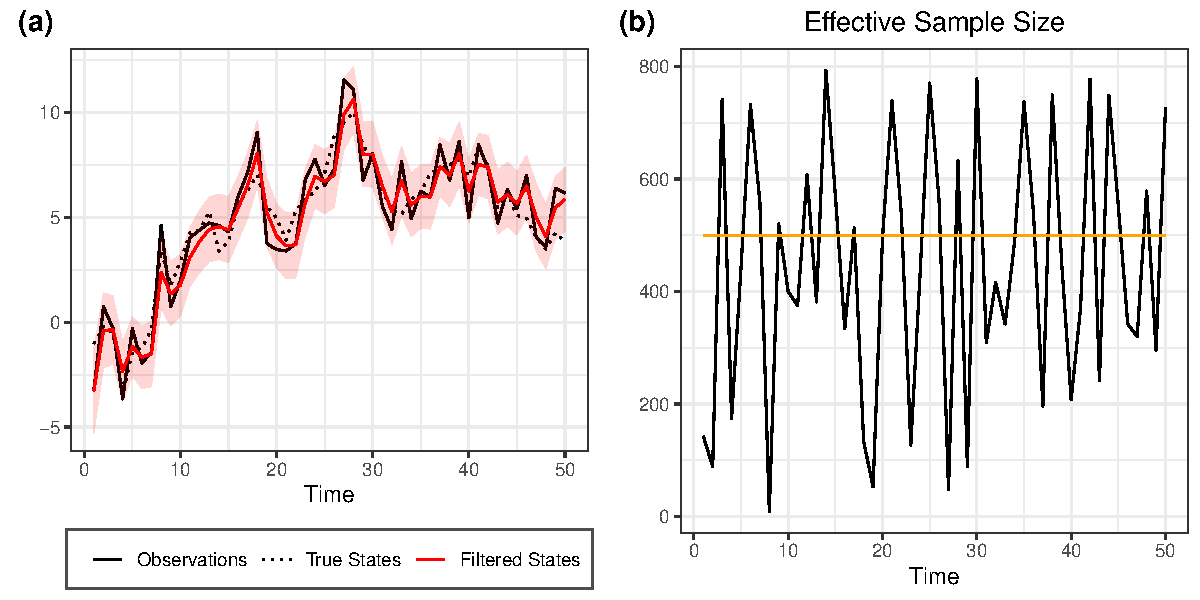
\includegraphics{new-draft_files/figure-latex/unnamed-chunk-13-1} 

}

\caption{a) PF Filtered States with credible interval (in red). b) Effective sample size (in black) with threshold (in yellow).}\label{fig:unnamed-chunk-13}
\end{figure}

Since the Random Walk plus Noise model allows for closed form solutions,
we want to compare the results of Boostrap Particle Filter(BPF) with
Kalman Filter(KF). As we can see from figure XX, when the number of
particles generated at any interaction increases the results for both
the estimated mean and the variance tend to converge {[}{[}SPIEGARE
PERCHE'{]}{]}. Moreover, comparing the Root Mean Square Errors of the
filtered states with respect to the true state values, when the sample
size increases the BPF decreases and, for large N, it reaches the
accuracy of the Kalman Filter.

\begin{longtable}[t]{cccc}
\caption{\label{tab:unnamed-chunk-15}Root Mean Square Errors}\\
\toprule
N & Threshold & KF & BPF\\
\midrule
100 & 0.5 & 0.879 & 0.888\\
1000 & 0.5 & 0.879 & 0.886\\
10000 & 0.5 & 0.879 & 0.878\\
\bottomrule
\end{longtable}

\begin{figure}[H]

{\centering 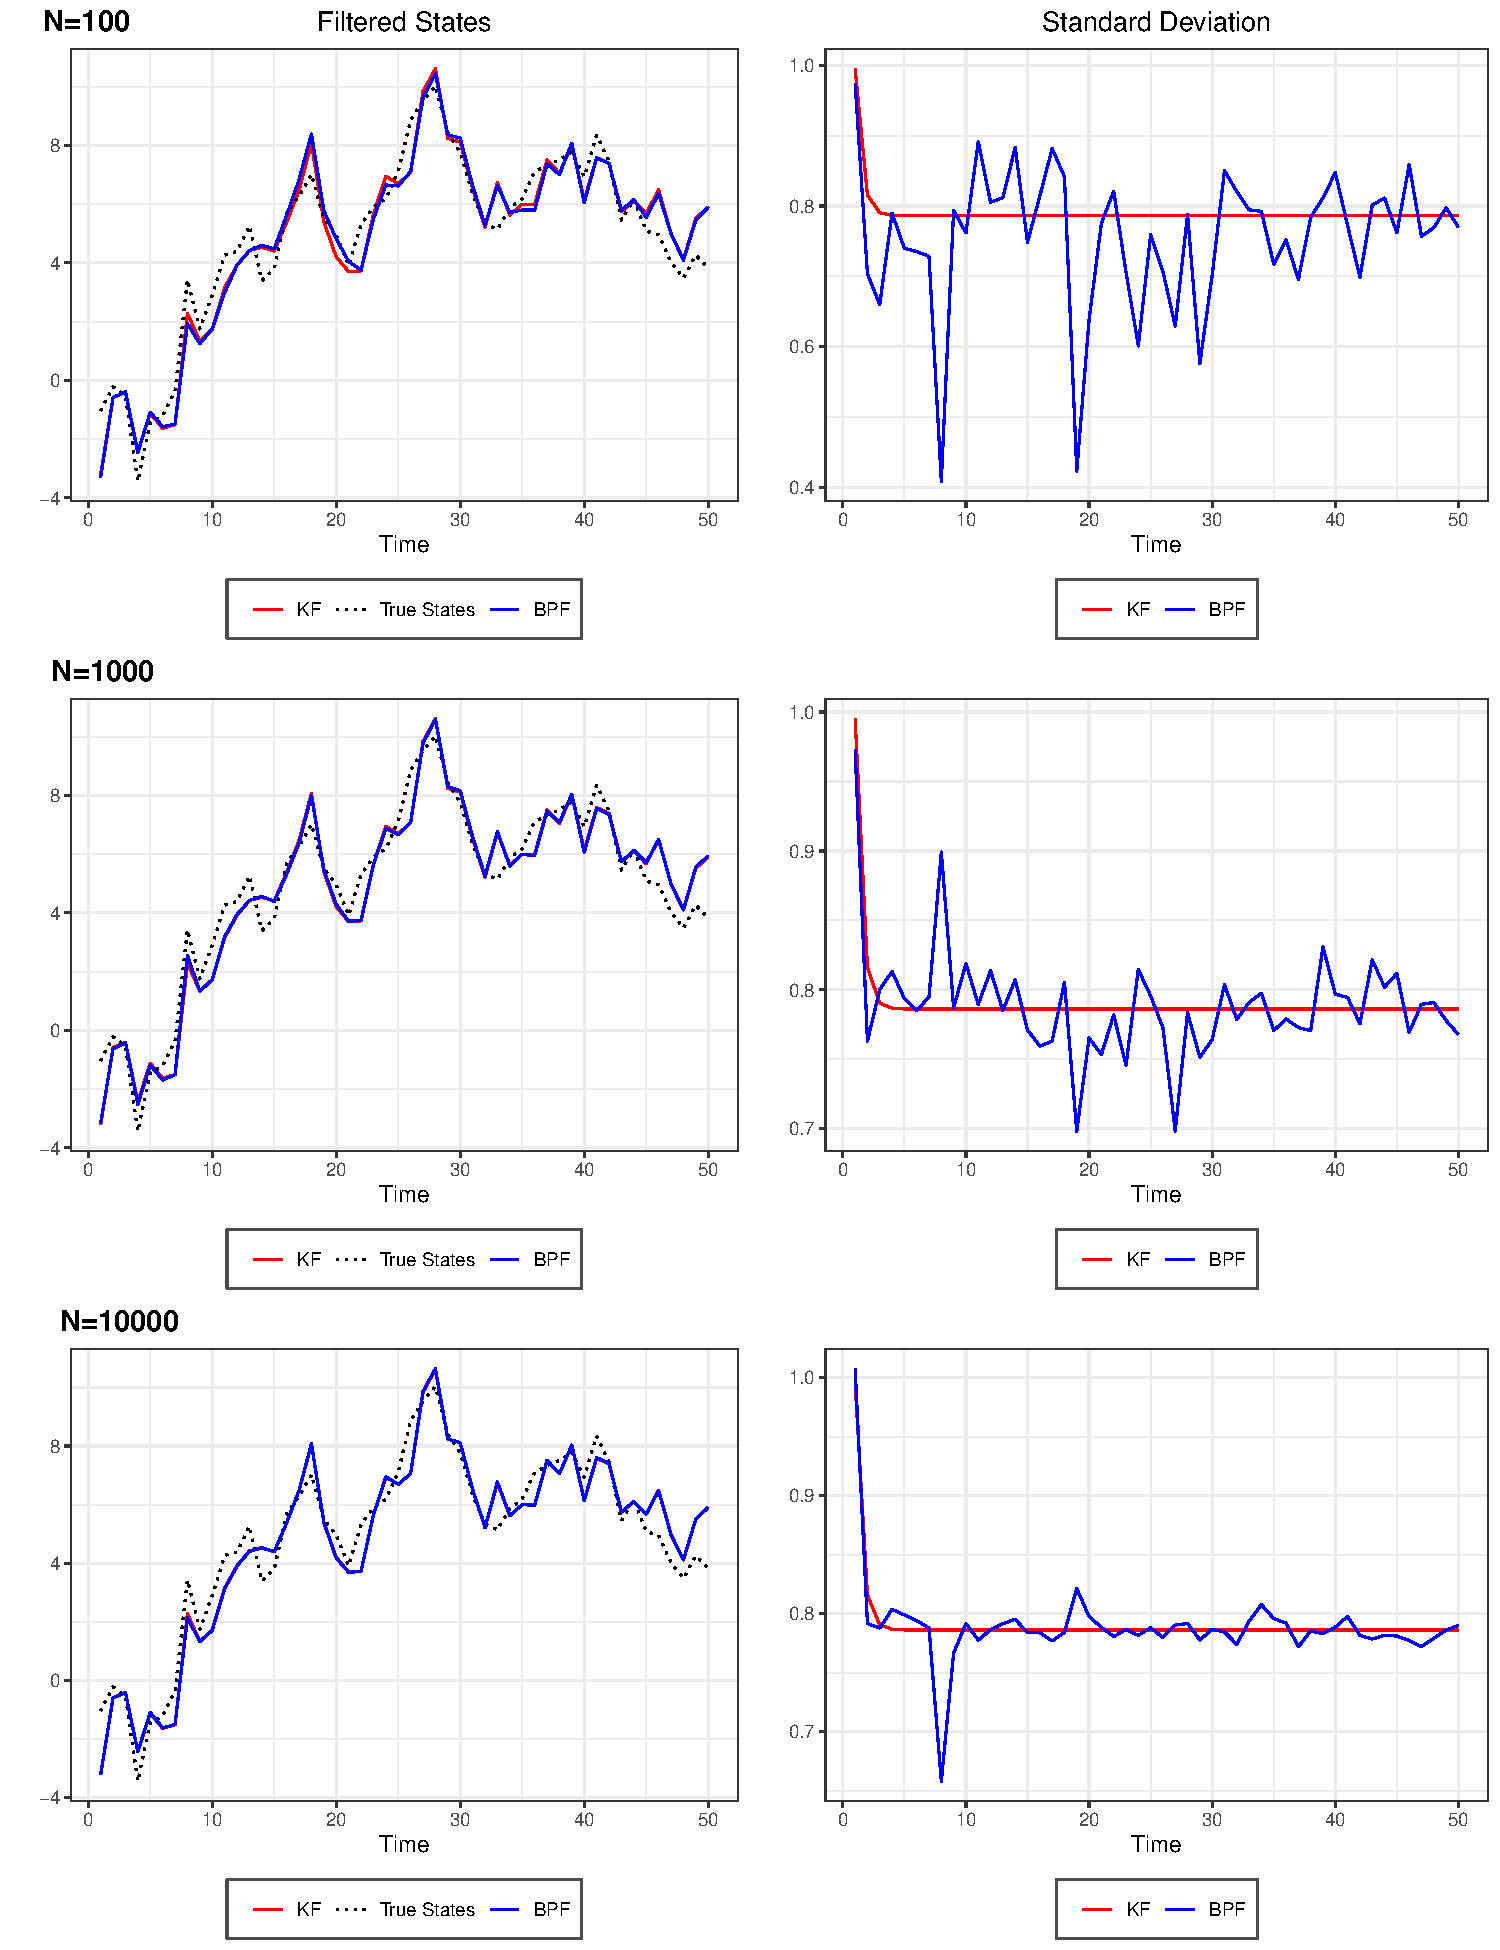
\includegraphics{new-draft_files/figure-latex/unnamed-chunk-16-1} 

}

\caption{Comparison Bootstrap Particle Filter(BPF) and Kalman Filter (KF) for increasing number of generated particles (N)}\label{fig:unnamed-chunk-16}
\end{figure}

\hfill\break

\subsection{Guided Particle Filter}

It is not always possible to sample sequentially from the correct
transition kernel. Moreover, even if it were possible, there exist a
proposal transition kernel that makes the algorithm more efficient. This
motivates the \textit{guided particle filter} (GPF), that can be
interpreted as a more general version of the GPF. In fact, with the GPF
it is possible, at each stage, to sample new states from a transition
kernel that differs from the correct one.~\\
Let \(P_t(x_{t-1},dx_t)\) be the correct kernel and consider a kernel
\(M_t(x_{t-1},dx_t)\) defined on the same measurable space of \(P_t\).
Moreover, let us assume that that \(P_t\) is absolutely continuous with
respect to
\(M_t\)\footnote{This condition is stronger than what would be needed for the existence of the importance weights in GPF, i.e., that  $P_t(x_{t-1},dx_t)\cdot f_t(y_t|x_t)\ll M_t(x_{t-1},dx_t)$. }
(i.e., \(P_t\ll M_t\)). If sampling occurs sequentially from this
kernel, the way in which weights are updated should differ from the BPF.
Consider equation \eqref{weight_updated_bpf} and let us reformulate it
for the GPF case. Here, the proposal distribution is not
\(\mathbb M_t(dx_{0:t}|y_{1:t})=\mathbb M_{t-1}(dx_{0:t-1}|y_{1:t-1})\cdot P_t(x_{t-1},dx_t)\)
anymore, but becomes
\(\mathbb M_t(dx_{0:t}|y_{1:t})=\mathbb M_{t-1}(dx_{0:t-1}|y_{1:t-1})\cdot M_t(x_{t-1},dx_t)\).
Hence: \begin{equation}
    \begin{split}
        w_t\propto&\frac{\mathbb P_t(dx_{0:t}|y_{1:t})}{\mathbb M_t(dx_{0:t}|y_{1:t})}\propto \frac{\mathbb P_{t-1}(dx_{0:t-1}|y_{1:t-1})\cdot P_t(x_{t-1},dx_t)\cdot f_t(y_t|x_t)}{\mathbb M_{t-1}(dx_{0:t-1}|y_{1:t-1})\cdot M_t(x_{t-1},dx_t)}=\\
        =&\underbrace{\frac{\mathbb P_{t-1}(dx_{0:t-1}|y_{0:t-1})}{\mathbb M_{t-1}(dx_{0:t-1}|y_{1:t-1})}}_{\hat w_{t-1}}\cdot\frac{P_t(x_{t-1},dx_t)\cdot f_t(y_t|x_t)}{ M_t(x_{t-1},dx_t)} =\hat w_{t-1}\cdot\underbrace{\frac{P_t(x_{t-1},dx_t)\cdot f_t(y_t|x_t)}{ M_t(x_{t-1},dx_t)}}_{\text{updating factor}}
    \end{split}\label{weight_updated_gpf}
\end{equation} Note that the updating factor is more complex that the
one of the BPF: in addition to the likelihood function \(f_t(y_t|x_t)\),
the fact that sampling occurs from a kernel different from the correct
ones requires the additional term
\(P_t(x_{t-1},dx_t)/M_t(x_{t-1},dx_t)\).~\\
We are now ready to establish, informally, the optimality result about
the transition kernel. Let us denote by
\(G_t=[P_t(x_{t-1},dx_t)\cdot f_t(y_t|x_t)dy_t]/M_t(x_{t-1},dx_t)\) the
\textit{incremental weights} (i.e., the updating factor) and by
\(M_t^*(x_{t-1},dx_t)\) the optimal kernel. It can be
proved\footnote{For a formal proof see \cite{**}, th. 10.1 p. 142.} that
the optimal kernel, i.e., the one that minimizes the variance of the
incremental weights \(G_t\) (and of the time \(t\) weights themselves),
is: \begin{equation}
    M_t^*(x_{t-1},dx_t)=\frac{1}{\int_{\mathcal X}P_t(x_{t-1},dx_t)\cdot f_t(y_t|x_t)} P_t(x_{t-1},dx_t)\cdot f_t(y_t|x_t)
\end{equation} Note that \(M_t^*\) is the conditional distribution of
\(x_t\) given \(x_{t-1}\) and
\(y_t\).\footnote{In fact, assuming that the $P_t$ admits a density $p_t$, applying Bayes rule, we have that $m_t(x_t|x_{t-1},y_t)\propto p_t(x_t|x_{t-1})\cdot f(y_t|x_t)$.}
The intuition for this result is apparent when considering equation
\eqref{weight_updated_gpf}: if \(M_t=M_t^*\), the updating factor
collapses to \(\int_{\mathcal X}P_t(x_{t-1},dx_t)\cdot f_t(y_t|x_t)\)
and information from the observed data are incorporated efficiently.\\
As a matter of fact, it is usually impossible to sample from the optimal
kernel and, in practice, it is replaced by its linear Gaussian
approximation. ~\\
The GPF can be resumed by the following steps.

\begin{enumerate}
    \item \textbf{Inital stage: }For $n=1,...,N$, at time 0 sample: $X_0^n\thicksim\mathbb M_0(dx_0)$ and set the un-normalized weights: 
    $$w_0^n=\frac{\mathbb P_0(dx_0)}{\mathbb M_0(dx_0)}.$$
    Then, the normalized weights are: $W_0^n:=\frac{w_0^n}{\sum_{m=1}^Nw_0^m}$.
    \item \textbf{For every $t=1,...T$:}
    \begin{enumerate}
        \item \textbf{Resample} if $ESS(W_{t-1}^{1:N})<ESS_{min}$:
\begin{enumerate}
    \item Multinomial sampling for the indexes $(A_t^n)_n$ with probabilities given by $(W_{t-1}^n)_n$.
    \item Update weights as: $\hat w_{t-1}^n = 1$ for $n=1,...,N$.
\end{enumerate}
\textbf{Otherwise, } 
\begin{enumerate}
    \item Set the indexes: $A_t^{n}=n$ for $n=1,...,N$
    \item Set the weights: $\hat w_{t-1}^n = w_{t-1}$ for $n=1,...,N$.
\end{enumerate}
\item Sample the future states from the transition kernel: $X_t^n\thicksim M_t(X_{t-1}^{A_t^n},dx_t)$ for $n=1,...,N$.
\item Update the un-normalized weights, for $n=1,...,N$:
\begin{equation*}
    w_t^n=\hat w_{t-1}^n\cdot \frac{P_t(X_{t-1}^{A_t^n},dx_t)\cdot f_t(y_t|X_t^n)}{ M_t(X_{t-1}^{A_t^n},dx_t)}.
\end{equation*}
\item Normalize the weights, for $n=1,...,N$:  $W_t^n:=\frac{w_t^n}{\sum_{m=1}^Nw_t^m}$.
    \end{enumerate}
\end{enumerate}

Note that \(\mathbb M_0(dx_0)\) is the initial sampling distribution,
that could differ from the correct one \(\mathbb P_0(dx_0)\).~\\
To conclude, one of the issues related to the BPF is the fact that new
states in \(t\) are sampled ignoring their likelihood given the future
observation \(y_t\). Hence, extractions from the ``correct" transition
kernel may be associated to low weights (small value for the
likelihood). Instead, the GPF allows to solve for this problem, defining
a proposal kernel that depends on the likelihood itself. Therefore, the
extraction of future states already incorporates the information given
by the data resulting in a more efficient procedure.

\section{Implementation}

\hfill\break
The Bootstrap Particle Filter Approach for the Random Walk plus Noise
Model described in Section XX can be improved accounting for the
observations in the importance transition density and it consists of
generating \(x_{t}\) from its conditional distribution given \(x_{t-1}\)
and \(y_{t}\). In the Normal model we are considering, the optimal
proposal will be a Normal density as well with mean and variance given
by \begin{align*}
\mu_{opt}=E(x_{t}|x_{t-1},y_{t})&=x_{t-1}+\frac{\tau^{2}}{\tau^{2}+\sigma^{2}}(y_{t}-x_{t-1})\\
\sigma_{opt}^{2}=V(x_{t}|x_{t-1},y_{t})&=\frac{\tau^{2}\sigma^{2}}{\tau^{2}+\sigma^{2}}
\end{align*} On the other hand, the incremental weights, using this
importance transition density, are proportional to the conditional
density of \(y_{t}\) given \(x_{t-1}=x_{t-1}^{(i)}\) , i.e
\(N(x_{t-1}^{(i)},\tau^{2}+\sigma^{2})\), evaluated at \(y_{t}\). In
other words the algorithm implemented in R is:

\begin{algorithm} GPF for Random Walk plus Noise Model
\begin{itemize}
\item Let $\{(x_{0},w_{0})^{(i)}\}_{i=1}^{N}$ summarizes $p(x_{0}|y_{0})$ such that, for example, $E(g(x_{0})|y_{0}) \approx \sum_{i=1}^{N}w_{0}^{(i)}g(x_{0}^{(i)})$. In particular, initialize $(x_{0}^{(1)},...,x_{0}^{(N)})$ from $N(m_{0},C_{0})$ and set $w_{0}^{(i)}=N^{-1} \ \forall \ i=1,...,N$.
\item Compute $\sigma_{opt}^{2}$ 
\item For $t=1,...,n$:
\begin{enumerate}
\item Compute $\mu_{opt}$
\item Draw $x_{t}^{(i)} \sim N(\mu_{opt},\sigma_{opt}^{2}) \ \ i=1,...,N$ such that $\{(x_{t},w_{t-1})^{(i)}\}_{i=1}^{N}$ summarizes $p(x_{t}|y_{t-1})$
\item Set $w_{t}^{(i)} = w_{t-1}^{(i)}f_{N}(y_{t};x_{t}^{(i)},\sigma^2+\tau^{2}) \ \ i=1,...,N$ such that $\{(x_{t},w_{t})^{(i)}\}_{i=1}^{N}$ summarizes $p(x_{t}|y_{t})$
\item if $ESS<N/2$ then
\begin{enumerate}
\item Draw a sample of size N, $(x_{t}^{(1)},...,x_{t}^{(N)})$, from the discrete distribution $P(x_{t}=x_{t}^{(i)})=w_{t}^{(i)},\ \ i=1,...,N$
\item Reset the weights: $w_{t}^{(i)}=N^{-1}$, $i=1,...,N$.
\end{enumerate}
\item Set $p(x_{t}|y_{t})=\sum_{i=1}^{N}w_{t}^{(i)}\delta_{x_{t}^{(i)}}$
\end{enumerate}
\end{itemize}
\end{algorithm}

The \texttt{GPFfun} function resume this passages.\\

\hrule
\hrule
\texttt{GPFfun(data,N,m0,C0,tau,sigma,r)}
\hrule

\textbf{Arguments}

\texttt{data} ~~the observed process. It has to be a vector or a
univariate time series.\\
\texttt{N} ~~number of particles generated at each step\\
\texttt{m0} ~~central value of the normal prior state distribution\\
\texttt{C0} ~~variance of the normal prior state distribution\\
\texttt{tau} ~~the standard deviation \(\tau\) in Equation (2)\\
\texttt{sigma} ~~the standard deviation \(\sigma\) in Equation (1)\\
\texttt{r} ~~ if present the threshold is set equal to \(N/r\)
otherwise, if missing, the threshold is set equal to \(N/2\)

\hrule
\hrule

\begin{Shaded}
\begin{Highlighting}[]
\NormalTok{GPFfun}\OtherTok{\textless{}{-}}\ControlFlowTok{function}\NormalTok{(data,N,m0,C0,tau,sigma,r)\{}
  \ControlFlowTok{if}\NormalTok{(}\FunctionTok{missing}\NormalTok{(r))\{r}\OtherTok{=}\DecValTok{2}\NormalTok{\}}\ControlFlowTok{else}\NormalTok{\{\}}
\NormalTok{  xs}\OtherTok{\textless{}{-}}\ConstantTok{NULL}
\NormalTok{  ws}\OtherTok{\textless{}{-}}\ConstantTok{NULL}
\NormalTok{  ess}\OtherTok{\textless{}{-}}\ConstantTok{NULL}
\NormalTok{  x  }\OtherTok{=} \FunctionTok{rnorm}\NormalTok{(N,m0,}\FunctionTok{sqrt}\NormalTok{(C0))}
\NormalTok{  importancesd}\OtherTok{\textless{}{-}}\FunctionTok{sqrt}\NormalTok{(tau }\SpecialCharTok{{-}}\NormalTok{ tau}\SpecialCharTok{\^{}}\DecValTok{2} \SpecialCharTok{/}\NormalTok{(tau }\SpecialCharTok{+}\NormalTok{ sigma))}
\NormalTok{  predsd }\OtherTok{\textless{}{-}} \FunctionTok{sqrt}\NormalTok{(sigma}\SpecialCharTok{+}\NormalTok{tau)}
\NormalTok{  w  }\OtherTok{=} \FunctionTok{rep}\NormalTok{(}\DecValTok{1}\SpecialCharTok{/}\NormalTok{N,N)}
  
  \ControlFlowTok{for}\NormalTok{(t }\ControlFlowTok{in} \DecValTok{1}\SpecialCharTok{:}\FunctionTok{length}\NormalTok{(data))\{}
    
\NormalTok{    means}\OtherTok{\textless{}{-}}\NormalTok{x}\SpecialCharTok{+}\NormalTok{(tau}\SpecialCharTok{/}\NormalTok{(tau}\SpecialCharTok{+}\NormalTok{sigma))}\SpecialCharTok{*}\NormalTok{(data[t]}\SpecialCharTok{{-}}\NormalTok{x)}
\NormalTok{    x}\OtherTok{\textless{}{-}}\FunctionTok{rnorm}\NormalTok{(N,means,importancesd)}
\NormalTok{    w1}\OtherTok{\textless{}{-}}\NormalTok{w}\SpecialCharTok{*}\FunctionTok{dnorm}\NormalTok{(data[t],x,predsd)}
    
\NormalTok{    w }\OtherTok{=}\NormalTok{ w1}\SpecialCharTok{/}\FunctionTok{sum}\NormalTok{(w1)}
\NormalTok{    ESS  }\OtherTok{=} \DecValTok{1}\SpecialCharTok{/}\FunctionTok{sum}\NormalTok{(w}\SpecialCharTok{\^{}}\DecValTok{2}\NormalTok{)}
    
    \ControlFlowTok{if}\NormalTok{(ESS}\SpecialCharTok{\textless{}}\NormalTok{(N}\SpecialCharTok{/}\NormalTok{r))\{}
\NormalTok{      index}\OtherTok{\textless{}{-}}\FunctionTok{sample}\NormalTok{(N,}\AttributeTok{size=}\NormalTok{N,}\AttributeTok{replace=}\NormalTok{T,}\AttributeTok{prob=}\NormalTok{w)}
\NormalTok{      x}\OtherTok{\textless{}{-}}\NormalTok{x[index]}
\NormalTok{      w}\OtherTok{\textless{}{-}}\FunctionTok{rep}\NormalTok{(}\DecValTok{1}\SpecialCharTok{/}\NormalTok{N,N)}
\NormalTok{    \}}\ControlFlowTok{else}\NormalTok{\{\}}
    
\NormalTok{    xs }\OtherTok{=} \FunctionTok{rbind}\NormalTok{(xs,x)}
\NormalTok{    ws }\OtherTok{=} \FunctionTok{rbind}\NormalTok{(ws,w)}
\NormalTok{    ess }\OtherTok{=}\FunctionTok{rbind}\NormalTok{(ess,ESS)}
\NormalTok{  \}}
  \FunctionTok{return}\NormalTok{(}\FunctionTok{list}\NormalTok{(}\AttributeTok{xs=}\NormalTok{xs,}\AttributeTok{ws=}\NormalTok{ws,}\AttributeTok{ess=}\NormalTok{ess))}
\NormalTok{\}}
\end{Highlighting}
\end{Shaded}

\begin{figure}[H]

{\centering 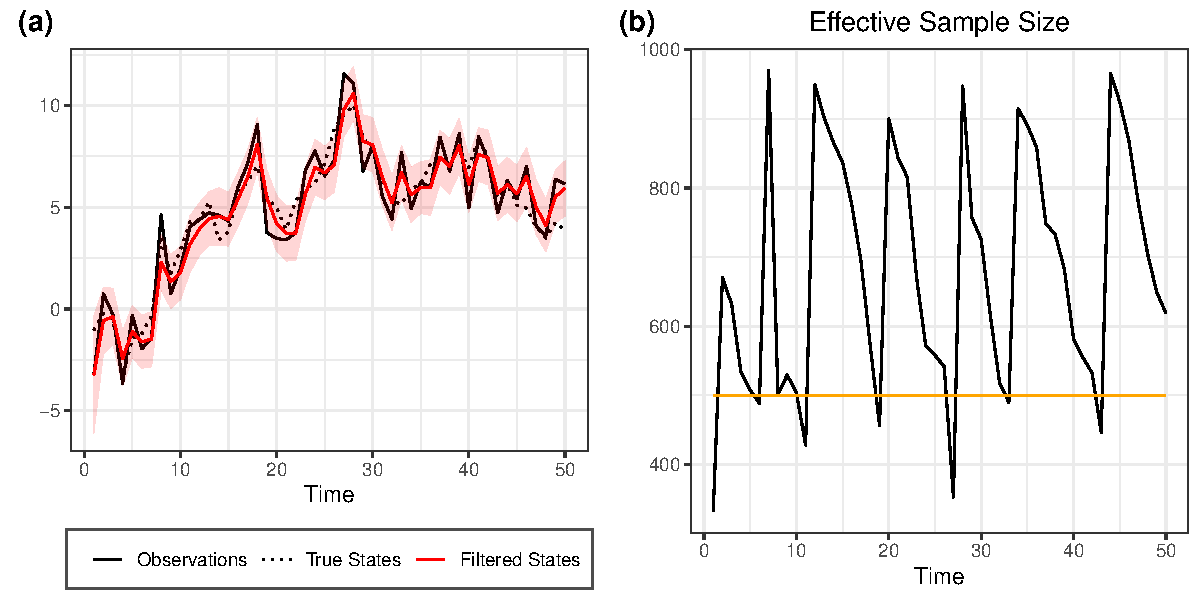
\includegraphics{new-draft_files/figure-latex/unnamed-chunk-19-1} 

}

\caption{a) GPF Filtered States with credible interval (in red). b) Effective sample size (in black) with threshold (in yellow).}\label{fig:unnamed-chunk-19}
\end{figure}

Let's provide directly a brief comparison between the Bootstrap Particle
Filter (BPF) and the Guided Particle Filter (GPF). As we can see from
the Figure XX, the Guided Particle Filter provides point estimates that
are slightly better with respect to the ones of the BPF, and this is
confirmed by the Table showing the RMSE. Moreover, also the variance is
better, suggesting for higher precision.

\begin{longtable}[t]{cccc}
\caption{\label{tab:unnamed-chunk-21}Root Mean Square Errors}\\
\toprule
N & Threshold & BPF & GPF\\
\midrule
1000 & 0.50 & 0.916 & 0.880\\
1000 & 0.25 & 0.895 & 0.862\\
1000 & 0.10 & 0.869 & 0.881\\
\bottomrule
\end{longtable}

\begin{figure}[H]

{\centering 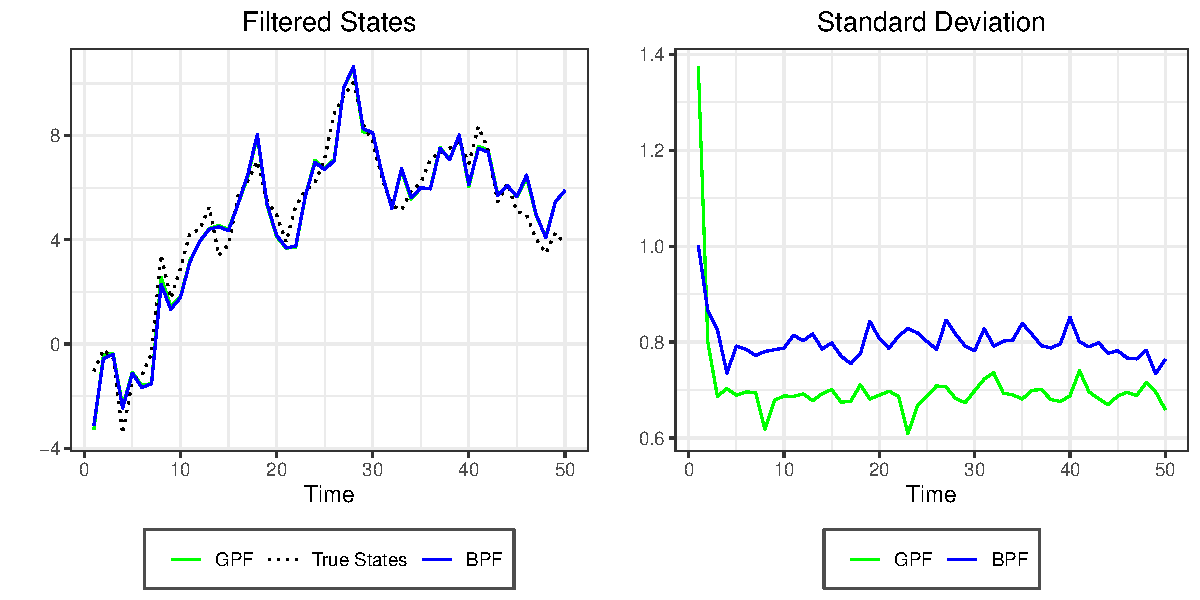
\includegraphics{new-draft_files/figure-latex/unnamed-chunk-22-1} 

}

\caption{Comparison Bootstrap Particle Filter(BPF) and Guided Particle Filter (GPF), number of generated particles N=1000}\label{fig:unnamed-chunk-22}
\end{figure}

\subsection{Auxiliary Particle Filter}

The \textit{auxiliary particle filter} (APF) constitutes a further
extension of the BPF. The GPF allowed to sample from a transition kernel
different from the correct ones. The APF, instead, allows to extract the
ancestor variables from an arbitrary distribution at the resampling
step.~\\
Let \(\eta_t:\mathcal X\rightarrow \mathbb R_+\) be a non-negative,
real-valued positive function, called \textit{auxiliary function}. At
time \(t\), when the resampling stage occurs, the multinomial
distribution for the indexes to be extracted can use probabilities that
differ from the weights in \(t-1\), \(W_{t-1}^n\). The new weights,
called \textit{auxiliary weights}, are computed as a transformation of
the original ones, denoted as \textit{inferential weights}, through the
auxiliary function: \begin{equation}
    \tilde W_t^n=\frac{W_t^n\cdot \eta_t(X_t^n)}{\sum_{m=1}^NW_t^m\cdot \eta_t(X_t^n)}
\end{equation} Note that the computation of the auxiliary weights is
done from the auto-normalized inferential ones. Additionally, note that
imposing \(\eta_t(x_t)=1\) we recover the GPF and the BPF as special
cases of the APF.\\
Clearly, inferential weights are updated by incorporating the fact that
resampling occurs according to different weights (the auxiliary ones):
\begin{equation}
    w_t^n=\frac{W_{t-1}^{A_t^n}}{\tilde W_{t-1}^{A_t^n}}G_t \label{apf_weights_up_}
\end{equation} where \(G_t\) is the incremental weight defined in the
section on GPF.~\\

To understand the logic of this sequential weight updating, consider
\eqref{weight_updated_gpf}. In particular, suppose that multinomial
resampling takes place at every stage and let
\(\tilde w_{t-1}:=w_{t-1}\cdot \eta_{t-1} (x_{t-1})\). Then:
\begin{equation}
    \begin{split}
        w_t\propto&\frac{\mathbb P_t(dx_{0:t}|y_{1:t})}{\mathbb M_t(dx_{0:t}|y_{1:t})}\propto \frac{\mathbb P_{t-1}(dx_{0:t-1}|y_{0:t-1})}{\mathbb M_{t-1}(dx_{0:t-1}|y_{1:t-1})\cdot \tilde w_{t-1}}\cdot\frac{P_t(x_{t-1},dx_t)\cdot f_t(y_t|x_t)}{ M_t(x_{t-1},dx_t)}\\
        =&\underbrace{\frac{\mathbb P_{t-1}(dx_{0:t-1}|y_{0:t-1})}{\mathbb M_{t-1}(dx_{0:t-1}|y_{1:t-1})}}_{w_{t-1}}\cdot\frac{1}{\tilde w_{t-1}}\cdot\frac{P_t(x_{t-1},dx_t)\cdot f_t(y_t|x_t)}{ M_t(x_{t-1},dx_t)}\\
        =&\frac{w_{t-1}}{ \tilde w_{t-1}}\cdot\frac{P_t(x_{t-1},dx_t)\cdot f_t(y_t|x_t)}{ M_t(x_{t-1},dx_t)}\label{weight_updated_apf}
    \end{split}
\end{equation} It is possible to derive an optimality result for the
auxiliary functions\footnote{Details in ***** th 10.2, p. 148}. In the
special case in which the transition kernel used for sampling
corresponds with the optimal one \(M_t^*\), the optimal auxiliary
function (i.e., the auxiliary function that minimizes the variance of
the inferential weights) becomes: \begin{equation}
    \eta_{t-1}^*(x_{t-1})=\int_\mathcal XP_t(x_{t-1},dx_t)f_t(y_t|x_t)
\end{equation} and is called \textit{perfectly adapted} auxiliary
function. In fact, if \(M_t=M_t^*\), then, expression
\eqref{weight_updated_apf} becomes: \begin{equation*}
    \begin{split}
        w_t\propto\frac{w_{t-1}}{ \tilde w_{t-1}}\cdot\frac{P_t(x_{t-1},dx_t)\cdot f_t(y_t|x_t)}{ M_t^*(x_{t-1},dx_t)}=\frac{1}{\eta_{t-1} (x_{t-1})}\cdot\int_\mathcal XP_t(x_{t-1},dx_t)f_t(y_t|x_t)
    \end{split}
\end{equation*} From the previous equation, it is clear that if
\(\eta_t=\eta_t^*\), the inferential weights are constant and their
variance is zero.\\
We can summarize the APF algorithm.

\begin{enumerate}
    \item \textbf{Inital stage: }
    \begin{enumerate}
        \item For $n=1,...,N$, at time 0 sample: $X_0^n\thicksim\mathbb M_0(dx_0)$ and set the un-normalized inferential weights: 
    $$w_0^n=\frac{\mathbb P_0(dx_0)}{\mathbb M_0(dx_0)}.$$
    Then, the normalized inferential weights are: $W_0^n:=\frac{w_0^n}{\sum_{m=1}^Nw_0^m}$.
    \item Compute the un-normalized auxiliary weights:
        $$\tilde w_0^n=w_0^n \cdot \eta_0(X_0^n)$$
        Then the normalized auxiliary weights are:
        $\tilde W_0^n:=\frac{\tilde w_0^n}{\sum_{m=1}^N\tilde w_0^m}$.
    \end{enumerate}
    \item \textbf{For every $t=1,...T$:}
    \begin{enumerate}
        \item \textbf{Resample} if $ESS( W_{t-1}^{1:N})<ESS_{min}$:
\begin{enumerate}
    \item Multinomial sampling for the indexes $(A_t^n)_n$ with probabilities given by $(\tilde W_{t-1}^n)_n$.
    \item Update weights as: $\hat w_{t-1}^n = \frac{W_{t-1}^{A_t^n}}{\tilde W_{t-1}^{A_t^n}} $ for $n=1,...,N$.
\end{enumerate}
\textbf{Otherwise, } 
\begin{enumerate}
    \item Set the indexes: $A_t^{n}=n$ for  $n=1,...,N$.
    \item Set the weights: $\hat w_{t-1}^n = w_{t-1}$ for $n=1,...,N$.
\end{enumerate}
\item Sample the future states from the transition kernel: $X_t^n\thicksim M_t(X_{t-1}^{A_t^n},dx_t)$ for $n=1,...,N$.
\item Update the un-normalized inferential weights, for $n=1,...,N$:
\begin{equation*}
    w_t^n=\hat w_{t-1}^n\cdot \frac{P_t(X_{t-1}^{A_t^n},dx_t)\cdot f_t(y_t|X_t^n)}{ M_t(X_{t-1}^{A_t^n},dx_t)}.
\end{equation*}
\item Normalize the inferential weights, for $n=1,...,N$:  $W_t^n:=\frac{w_t^n}{\sum_{m=1}^Nw_t^m}$.
\item Compute the un-normalized auxiliary weights, for $n=1,...,N$:
\begin{equation*}
 \tilde w_t^n=w_t^n \cdot \eta_t(X_t^n)
\end{equation*}
\item Normalize the auxiliary weights, for $n=1,...,N$:  $\tilde W_t^n:=\frac{\tilde w_t^n}{\sum_{m=1}^N\tilde w_t^m}$.\footnote{It is worth mentioning that the original APF included a final resampling step at the end of each iteration. However, our formulation is more efficient since having two resampling steps might introduce additional Monte Carlo variance. Se ***Johansen p. 120}
    \end{enumerate}
\end{enumerate}

However, it is worth noting that the optimality results both for the
kernel in the GPF and of the auxiliary in the APF, has two main
weaknesses:

\begin{itemize}
    \item it is not clear that what is optimal at time $t$ remains such at future stages. In other words, it is not truly clear how the minimization of the variance of the inferential weights at each stage affect the efficiency of the PF estimators;
    \item both the choice of $M_t$ and of $\eta_t$ affect the way in which weights are computed and, indirectly, the decision to resample in the future. It is difficult to take also this indirect effect into account when evaluating the  overall efficiency of the algorithm.
\end{itemize}

For illustration purposes, we are going implement an auxiliary particle
filter with auxiliary function
\(g(x_{t-1})=E(x_{t}|x_{t-1})=x_{t-1}\).\\

\begin{algorithm} APF for Random Walk plus Noise Model
\begin{itemize}
\item Let $\{(x_{0},w_{0})^{(i)}\}_{i=1}^{N}$ summarizes $p(x_{0}|y_{0})$ such that, for example, $E(g(x_{0})|y_{0}) \approx \sum_{i=1}^{N}w_{0}^{(i)}g(x_{0}^{(i)})$. In particular, initialize $(x_{0}^{(1)},...,x_{0}^{(N)})$ from $N(m_{0},C_{0})$ and set $w_{0}^{(i)}=N^{-1} \ \forall \ i=1,...,N$.
\item For $t=1,...,n$:
\begin{enumerate}
\item For $k=1,...,N$:
\begin{enumerate}
\item Draw $I_{k}$ with $P(I_{k}) \propto w_{t-1}^{(i)}f(y_{t}|g(x_{t-1}^{(i)})) $
\item Draw $x_{t}^{(k)} \sim N(x_{t-1}^{(I_{k})},\tau^2)$
\item Set  $\tilde{w}_{t}^{(k)} = \frac{f_{N}(y_{t}|x_{t}^{(k)})}{f_{N}(y_{t}|g(x_{t-1}^{(I_{k})}))}$
\end{enumerate}
\item Normalize the weights: $w_{t}^{(i)}=\frac{\tilde{w}_{t}^{(i)}}{\sum_{j=1}^{N}(\tilde{w}_{t}^{(j)})}$
\item Compute $ESS=\Bigg(\sum_{i=1}^{N}(w_{t}^{(i)})^{2}\Bigg)^{-1}$
\item if $ESS<N/2$ then
\begin{enumerate}
\item Draw a sample of size N, $(x_{t}^{(1)},...,x_{t}^{(N)})$, from the discrete distribution $P(x_{t}=x_{t}^{(i)})=w_{t}^{(i)},\ \ i=1,...,N$
\item Reset the weights: $w_{t}^{(i)}=N^{-1}$, $i=1,...,N$.
\end{enumerate}
\item Set $p(x_{t}|y_{1:t})=\sum_{i=1}^{N}w_{t}^{(i)}\delta_{x_{t}^{(i)}}$
\end{enumerate}
\end{itemize}
\end{algorithm}

The \texttt{APFfun} function resume this passages.\\

\hrule
\hrule

\hfill\break
\texttt{APFfun(data,N,m0,C0,tau,sigma,r)}

\hrule

\hfill\break
\textbf{Arguments}

\texttt{data} ~~the observed process. It has to be a vector or a
univariate time series.\\
\texttt{N} ~~number of particles generated at each step\\
\texttt{m0} ~~central value of the normal prior state distribution\\
\texttt{C0} ~~variance of the normal prior state distribution\\
\texttt{tau} ~~the standard deviation \(\tau\) in Equation (2)\\
\texttt{sigma} ~~the standard deviation \(\sigma\) in Equation (1)\\
\texttt{r} ~~ if present the threshold is set equal to \(N/r\)
otherwise, if missing, the threshold is set equal to \(N/2\)

\hrule
\hrule

\begin{Shaded}
\begin{Highlighting}[]
\NormalTok{APFfun}\OtherTok{\textless{}{-}}\ControlFlowTok{function}\NormalTok{(data,N,m0,C0,tau,sigma,r)\{}
  \ControlFlowTok{if}\NormalTok{(}\FunctionTok{missing}\NormalTok{(r))\{r}\OtherTok{=}\DecValTok{2}\NormalTok{\}}\ControlFlowTok{else}\NormalTok{\{\}}
\NormalTok{  xs}\OtherTok{\textless{}{-}}\ConstantTok{NULL}
\NormalTok{  ws}\OtherTok{\textless{}{-}}\ConstantTok{NULL}
\NormalTok{  ess}\OtherTok{\textless{}{-}}\ConstantTok{NULL}
\NormalTok{  x  }\OtherTok{=} \FunctionTok{rnorm}\NormalTok{(N,m0,}\FunctionTok{sqrt}\NormalTok{(C0))}
\NormalTok{  w  }\OtherTok{=} \FunctionTok{rep}\NormalTok{(}\DecValTok{1}\SpecialCharTok{/}\NormalTok{N,N)}
  
  \ControlFlowTok{for}\NormalTok{(t }\ControlFlowTok{in} \DecValTok{1}\SpecialCharTok{:}\FunctionTok{length}\NormalTok{(data))\{}
    
\NormalTok{    weight }\OtherTok{=}\NormalTok{ w}\SpecialCharTok{*}\FunctionTok{dnorm}\NormalTok{(data[t],x,sigma)}
\NormalTok{    k   }\OtherTok{=} \FunctionTok{sample}\NormalTok{(}\DecValTok{1}\SpecialCharTok{:}\NormalTok{N,}\AttributeTok{size=}\NormalTok{N,}\AttributeTok{replace=}\ConstantTok{TRUE}\NormalTok{,}\AttributeTok{prob=}\NormalTok{weight)}
\NormalTok{    x1   }\OtherTok{=} \FunctionTok{rnorm}\NormalTok{(N,x[k],tau)}
\NormalTok{    lw  }\OtherTok{=} \FunctionTok{dnorm}\NormalTok{(data[t],x1,sigma,}\AttributeTok{log=}\ConstantTok{TRUE}\NormalTok{)}\SpecialCharTok{{-}}\FunctionTok{dnorm}\NormalTok{(data[t],x[k],sigma,}\AttributeTok{log=}\ConstantTok{TRUE}\NormalTok{)}
\NormalTok{    w   }\OtherTok{=} \FunctionTok{exp}\NormalTok{(lw)}
\NormalTok{    w   }\OtherTok{=}\NormalTok{ w}\SpecialCharTok{/}\FunctionTok{sum}\NormalTok{(w)}
\NormalTok{    ESS  }\OtherTok{=} \DecValTok{1}\SpecialCharTok{/}\FunctionTok{sum}\NormalTok{(w}\SpecialCharTok{\^{}}\DecValTok{2}\NormalTok{)}
    
    \ControlFlowTok{if}\NormalTok{(ESS}\SpecialCharTok{\textless{}}\NormalTok{(N}\SpecialCharTok{/}\NormalTok{r))\{}
\NormalTok{      index}\OtherTok{\textless{}{-}}\FunctionTok{sample}\NormalTok{(N,}\AttributeTok{size=}\NormalTok{N,}\AttributeTok{replace=}\NormalTok{T,}\AttributeTok{prob=}\NormalTok{w)}
\NormalTok{      x1}\OtherTok{\textless{}{-}}\NormalTok{x1[index]}
\NormalTok{      w}\OtherTok{\textless{}{-}}\FunctionTok{rep}\NormalTok{(}\DecValTok{1}\SpecialCharTok{/}\NormalTok{N,N)}
\NormalTok{    \}}\ControlFlowTok{else}\NormalTok{\{\}}
    
\NormalTok{    x }\OtherTok{\textless{}{-}}\NormalTok{ x1}
\NormalTok{    xs }\OtherTok{=} \FunctionTok{rbind}\NormalTok{(xs,x)}
\NormalTok{    ws }\OtherTok{=} \FunctionTok{rbind}\NormalTok{(ws,w)}
\NormalTok{    ess }\OtherTok{=}\FunctionTok{rbind}\NormalTok{(ess,ESS)}
    
\NormalTok{  \}}
  \FunctionTok{return}\NormalTok{(}\FunctionTok{list}\NormalTok{(}\AttributeTok{xs=}\NormalTok{xs,}\AttributeTok{ws=}\NormalTok{ws,}\AttributeTok{ess=}\NormalTok{ess))}
\NormalTok{\}}
\end{Highlighting}
\end{Shaded}

\begin{figure}[H]

{\centering 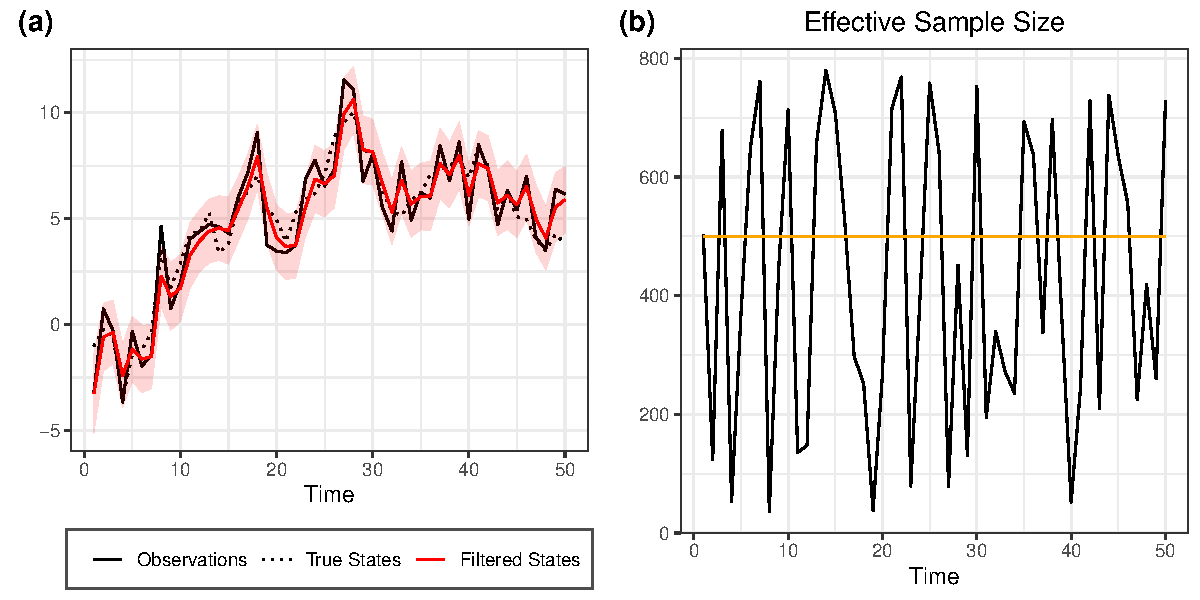
\includegraphics{new-draft_files/figure-latex/unnamed-chunk-25-1} 

}

\caption{a) APF Filtered States with credible interval (in red). b) Effective sample size (in black) with threshold (in yellow).}\label{fig:unnamed-chunk-25}
\end{figure}

Let's compare the Auxiliary Particle Filter (APF) and the Bootstrap
Particle Filter (BPF).

\begin{figure}[H]

{\centering 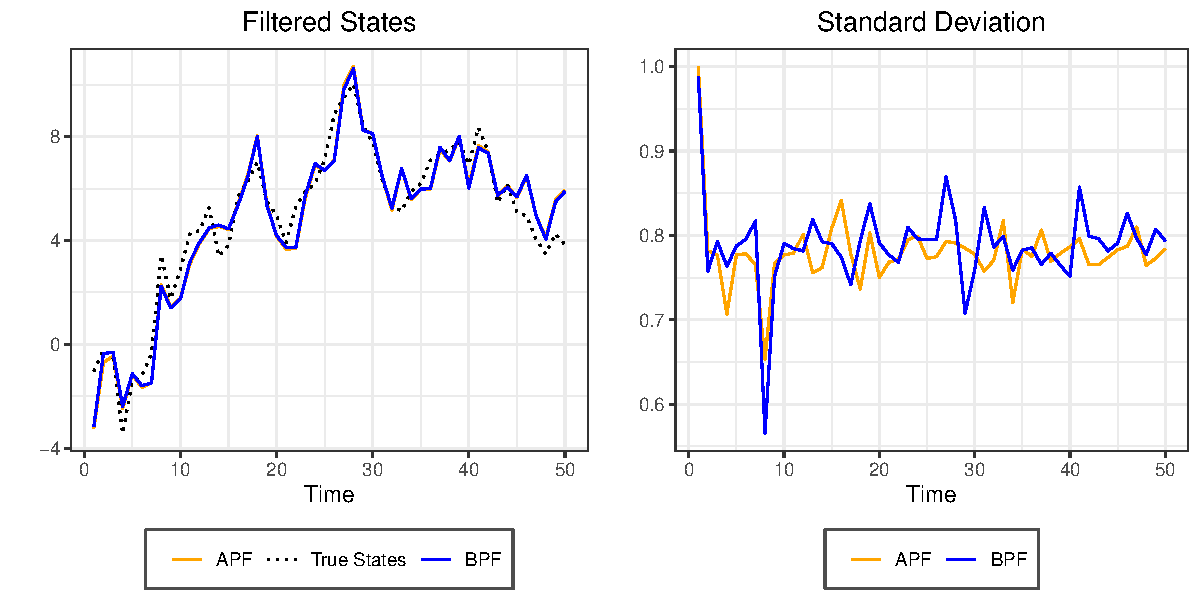
\includegraphics{new-draft_files/figure-latex/unnamed-chunk-26-1} 

}

\caption{Comparison Bootstrap Particle Filter(BPF) and Guided Particle Filter (GPF), number of generated particles N=1000}\label{fig:unnamed-chunk-26}
\end{figure}

\begin{longtable}[t]{cccc}
\caption{\label{tab:unnamed-chunk-28}Root Mean Square Errors}\\
\toprule
N & Threshold & BPF & APF\\
\midrule
1000 & 0.50 & 0.885 & 0.875\\
1000 & 0.25 & 0.893 & 0.892\\
1000 & 0.10 & 0.855 & 0.870\\
\bottomrule
\end{longtable}

\begin{Shaded}
\begin{Highlighting}[]
\NormalTok{APFoptfun}\OtherTok{\textless{}{-}}\ControlFlowTok{function}\NormalTok{(data,N,m0,C0,tau,sigma,r)\{}
  \ControlFlowTok{if}\NormalTok{(}\FunctionTok{missing}\NormalTok{(r))\{r}\OtherTok{=}\DecValTok{2}\NormalTok{\}}\ControlFlowTok{else}\NormalTok{\{\}}
\NormalTok{  xs}\OtherTok{\textless{}{-}}\ConstantTok{NULL}
\NormalTok{  ws}\OtherTok{\textless{}{-}}\ConstantTok{NULL}
\NormalTok{  ess}\OtherTok{\textless{}{-}}\ConstantTok{NULL}
\NormalTok{  x  }\OtherTok{=} \FunctionTok{rnorm}\NormalTok{(N,m0,}\FunctionTok{sqrt}\NormalTok{(C0))}
\NormalTok{  importancesd}\OtherTok{\textless{}{-}}\FunctionTok{sqrt}\NormalTok{(tau }\SpecialCharTok{{-}}\NormalTok{ tau}\SpecialCharTok{\^{}}\DecValTok{2} \SpecialCharTok{/}\NormalTok{(tau }\SpecialCharTok{+}\NormalTok{ sigma))}
\NormalTok{  predsd }\OtherTok{\textless{}{-}} \FunctionTok{sqrt}\NormalTok{(sigma}\SpecialCharTok{+}\NormalTok{tau)}
\NormalTok{  w  }\OtherTok{=} \FunctionTok{rep}\NormalTok{(}\DecValTok{1}\SpecialCharTok{/}\NormalTok{N,N)}
  
  \ControlFlowTok{for}\NormalTok{(t }\ControlFlowTok{in} \DecValTok{1}\SpecialCharTok{:}\FunctionTok{length}\NormalTok{(data))\{}
\NormalTok{    ESS  }\OtherTok{=} \DecValTok{1}\SpecialCharTok{/}\FunctionTok{sum}\NormalTok{(w}\SpecialCharTok{\^{}}\DecValTok{2}\NormalTok{)}
    
    \ControlFlowTok{if}\NormalTok{(ESS}\SpecialCharTok{\textless{}}\NormalTok{(N}\SpecialCharTok{/}\NormalTok{r))\{}
\NormalTok{    weight }\OtherTok{=}\NormalTok{ w}\SpecialCharTok{*}\FunctionTok{dnorm}\NormalTok{(data[t],x,predsd)}
\NormalTok{    k   }\OtherTok{=} \FunctionTok{sample}\NormalTok{(}\DecValTok{1}\SpecialCharTok{:}\NormalTok{N,}\AttributeTok{size=}\NormalTok{N,}\AttributeTok{replace=}\ConstantTok{TRUE}\NormalTok{,}\AttributeTok{prob=}\NormalTok{weight)}
\NormalTok{    \}}\ControlFlowTok{else}\NormalTok{\{}
\NormalTok{    weight }\OtherTok{=} \FunctionTok{rep}\NormalTok{(}\DecValTok{1}\SpecialCharTok{/}\NormalTok{N,N)}
\NormalTok{    k   }\OtherTok{=} \FunctionTok{sample}\NormalTok{(}\DecValTok{1}\SpecialCharTok{:}\NormalTok{N,}\AttributeTok{size=}\NormalTok{N,}\AttributeTok{replace=}\ConstantTok{TRUE}\NormalTok{,}\AttributeTok{prob=}\NormalTok{weight)}
\NormalTok{    \}}
    
\NormalTok{    means}\OtherTok{\textless{}{-}}\NormalTok{x[k]}\SpecialCharTok{+}\NormalTok{(tau}\SpecialCharTok{/}\NormalTok{(tau}\SpecialCharTok{+}\NormalTok{sigma))}\SpecialCharTok{*}\NormalTok{(data[t]}\SpecialCharTok{{-}}\NormalTok{x[k])}
\NormalTok{    x1   }\OtherTok{=} \FunctionTok{rnorm}\NormalTok{(N,means,importancesd)}
\NormalTok{    lw  }\OtherTok{=} \FunctionTok{dnorm}\NormalTok{(data[t],x1,predsd,}\AttributeTok{log=}\ConstantTok{TRUE}\NormalTok{)}\SpecialCharTok{{-}}\FunctionTok{dnorm}\NormalTok{(data[t],x[k],predsd,}\AttributeTok{log=}\ConstantTok{TRUE}\NormalTok{)}
\NormalTok{    w   }\OtherTok{=} \FunctionTok{exp}\NormalTok{(lw)}
\NormalTok{    w   }\OtherTok{=}\NormalTok{ w}\SpecialCharTok{/}\FunctionTok{sum}\NormalTok{(w)}
\NormalTok{    x }\OtherTok{\textless{}{-}}\NormalTok{ x1}
   
    
\NormalTok{    xs }\OtherTok{=} \FunctionTok{rbind}\NormalTok{(xs,x)}
\NormalTok{    ws }\OtherTok{=} \FunctionTok{rbind}\NormalTok{(ws,w)}
\NormalTok{    ess }\OtherTok{=}\FunctionTok{rbind}\NormalTok{(ess,ESS)}
    
\NormalTok{  \}}
  \FunctionTok{return}\NormalTok{(}\FunctionTok{list}\NormalTok{(}\AttributeTok{xs=}\NormalTok{xs,}\AttributeTok{ws=}\NormalTok{ws,}\AttributeTok{ess=}\NormalTok{ess))}
\NormalTok{\}}
\end{Highlighting}
\end{Shaded}

\begin{figure}[H]

{\centering 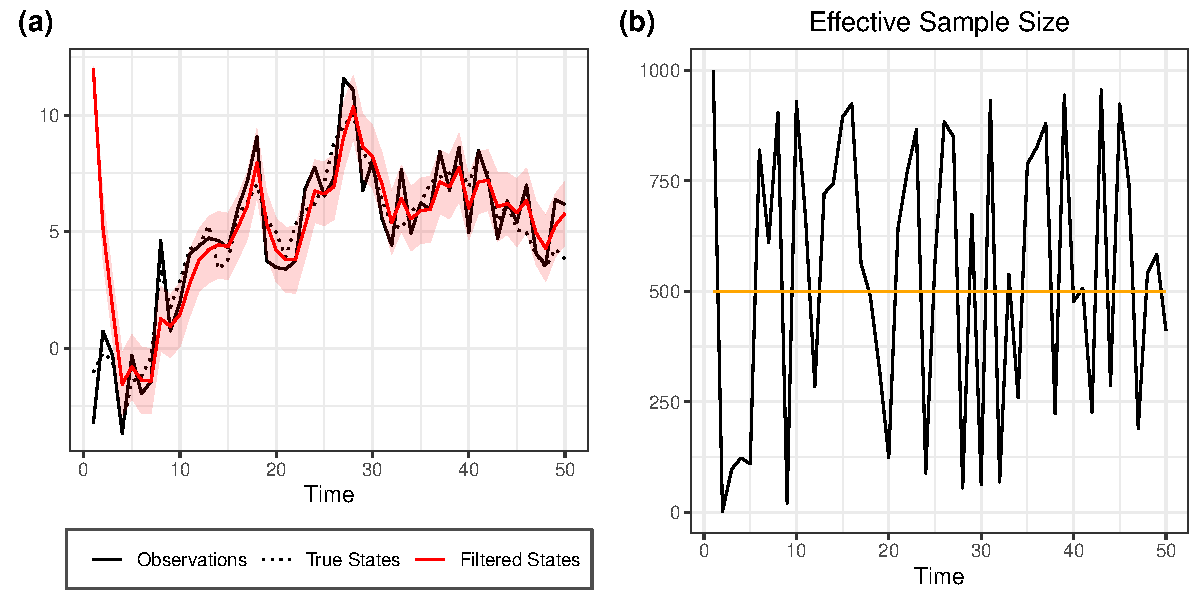
\includegraphics{new-draft_files/figure-latex/unnamed-chunk-31-1} 

}

\caption{a) APF Filtered States with credible interval (in red). b) Effective sample size (in black) with threshold (in yellow).}\label{fig:unnamed-chunk-31}
\end{figure}

\section{Liu and West Filter}\label{pf_lui_west}

Let us consider a more general state-space model, where the state vector
includes a time-constant parameter vector \(\psi \in \Psi\), where
\(\Psi\) is the parameter space. Since we can interpret the parameter as
a state with the law of motion \(\psi_t=\psi_{t-1}=\psi\), then it is
possible to adopt a PF algorithm to estimate \(\psi\).\\
However, being \(\psi\) constant over time, it is meaningless to sample
its values sequentially: the first extraction of \(\psi\) at the initial
stage 0 (i.e., \(\psi_0^n\)) generates a constant path of particles for
the parameter (\(\psi_t^n=\psi_0^n\)).
\footnote{To be more precise, at the resampling step, also $\psi^n$ is resampled, but the possible values that it may take are the $N$ ones obtained at the initial time 0 extraction.}\\
Therefore, Liu and West (2001) proposed a modified particle filter,
called \textit{Liu and West filter} (LWF) that allows to resample the
parameter over time from a continuous distribution. In this way, at
every time, the support of \(\psi\) is not limited to the initially
sampled \(N\) values.\\
Here, we describe the LWF that makes use of the normal distribution to
sample sequentially the parameter. Moreover, consider the simpler
version of the bootstrap
filter.\footnote{Clearly, the LWF can be also used within the more general frameweorks of the GPF and the APF.}\\
Let the transition kernel and the likelihood depend on the parameter
\(\psi\) (i.e., \(P_t(x_{t-1},dx_t;\psi)\) and \(f_t(y_t|x_t;\psi)\))
and let \$\pi(\cdot) \$ be the prior distribution for the parameter
\(\psi\).\\
The LWF can be described by the following algorithm.

\begin{enumerate}
    \item \textbf{Inital stage: }For $n=1,...,N$, at time 0 sample: $X_0^n\thicksim\mathbb P_0(dx_0)$ and $\psi_0^n\thicksim \pi(\psi_0)$.
    
    Then, set the un-normalized weights $w_0^n=1$.
    
    Hence, the normalized weights are: $W_0^n=\frac{1}{N}$.
    \item \textbf{For every $t=1,...T$:}
    \begin{enumerate}
        \item \textbf{Resample} if $ESS(W_{t-1}^{1:N})<ESS_{min}$:
\begin{enumerate}
    \item Multinomial sampling for the indexes $(A_t^n)_n$ with probabilities given by $(W_{t-1}^n)_{n}$.
    \item Update weights as: $\hat w_{t-1}^n = 1$ for $n=1,...,N$.
\end{enumerate}
\textbf{Otherwise, } 
\begin{enumerate}
    \item Set the indexes: $A_t^{n}=n$ for  $n=1,...,N$
    \item Set the weights: $\hat w_{t-1}^n = w_{t-1}$ for $n=1,...,N$.
\end{enumerate}
\item \textbf{Extracting new parameter values:}
\begin{enumerate}
    \item Compute the weighted average and the variance for the parameters, respectively: $\bar \psi = \sum_{n=1}^N W_{t-1}^n\psi^n$, $\Omega = \sum_{n=1}^N W_{t-1}^n(\psi^n-\bar \psi)^2$.
    \item Compute: $m^n=a\cdot  \psi^n+(1-a)\cdot \bar \psi$ for $n=1,...,N$.
    \item Draw new parameters: $\psi^n\thicksim \mathcal N\big(m^{A_t^n},h^2\cdot \Omega\big)$ for $n=1,...,N$.
\end{enumerate}
\item Sample future states from the transition kernel: $X_t^n\thicksim P_t(X_{t-1}^{A_t^n},dx_t; \psi^n)$ for $n=1,...,N$.
\item Update the un-normalized weights through the likelihood function, for $n=1,...,N$:
\begin{equation*}
    w_t^n=\hat w_{t-1}^n\cdot f_t(y_t|X_t^n;\psi^n).
\end{equation*}
\item Normalize the weights, for $n=1,...,N$:  $W_t^n:=\frac{w_t^n}{\sum_{m=1}^Nw_t^m}$.
    \end{enumerate}
\end{enumerate}

At the initial step, \(N\) states and \(N\) parameter values are sampled
independently, respectively, from \(\mathbb P_0\) and \(\pi\) and the
particle weights are set to be constant, as usual.\\
Then, at each iteration (time \(t\)), the decision to resample is done
according to the \(ESS\) criterion and indexes are extracted from a
multinomial distribution. However, in the LWF both previous periods
states and parameters are resampled.\\
Meanwhile, to extract the next period states and parameters it is
necessary, firstly, to sample the new \(N\) parameter values. Let
\(\bar \psi\) be the weighted average of the parameter values and
\(\Omega\) be their variance (the weights used to compute this mean and
variance are the previous period inferential ones,
i.e.~\(W_{t-1}^n\)).~\\
The algorithm suggests to sample new values for the parameters from a
continuous distribution, i.e., a Normal centered at the (resampled)
values \(m^{A_t^n}\) with variance \(h^2\cdot \Omega\) where \(m^n\) is
a convex combination of the sample mean \(\bar\psi\) and the actual
extraction of \(\psi^n\) with coefficient \(a\in (0,1)\) and \(h\) is a
scalar such that \(a^2+h^2=1\). While it would be more intuitively
immediate to sample new parameters from a Normal density centered at the
previously sampled values (i.e., \(\psi^n\)), this would increase the
variance of \(\psi\) over time.\\
In fact, let
\(\pi_{t-1}^N(\psi)=\sum_{n=1}^N \hat W_{t-1}^{A_t^{n}}\cdot \mathcal N(\psi^{A_t^{n}},\Omega)\)\footnote{Big hat-weights $ \hat W_{t-1}^{A_t^{n}}$ are the normalized weights after the resampling stage, equal to $1/N$ if resampling takes place, $W_{t-1}^n$ otherwise.}
be the empirical distribution of the parameters. From the law of
iterated expectation and total variance, we
obtain:\footnote{For completeness, we specify that the first expected value in the law of iterated expectations and total variances is with respect to the distribution of the indexes and the second one with respect to each of the Normal distributions centered at $\psi^{A_t^{n}}$.}
\begin{equation*}
    \begin{split}
        \mathbb E_{\pi_{t-1}^N} ( \psi)=& \mathbb E\big[\mathbb E( \psi|A_t^{n})\big]=\mathbb E\big[\psi^{A_t^{n}}\big]=\bar \psi\\
        Var_{\pi_{t-1}^N} ( \psi)=&Var\big[\mathbb E( \psi|A_t^{n})\big]+\mathbb E\big[Var( \psi|A_t^{n})\big]=Var\big[\psi^{A_t^{n}}\big]+\mathbb E\big[\Omega\big]=2\cdot\Omega
    \end{split}
\end{equation*} Hence, while the mean is preserved, the variance
increases at each iteration. Instead, sampling from the distribution
proposed by Liu and West
\(\mathcal N\big(m^{A_t^n},h^2\cdot \Omega\big)\) preserves both the
mean and the variance of the parameters over time.\\
Let
\(\tilde \pi_{t-1}^N(\psi)=\sum_{n=1}^N \hat W_{t-1}^{A_t^{n}}\cdot \mathcal N\big(m^{A_t^n},h^2\cdot \Omega\big)\).
Hence: \begin{equation*}
    \begin{split}
        \mathbb E_{\tilde \pi_{t-1}^N} ( \psi)=& \mathbb E\big[\mathbb E( \psi|A_t^{n})\big]=\mathbb E\big[m^{A_t^n}\big]=\mathbb E\big[a\cdot \psi^{A_t^n}+(1-a)\cdot \bar \psi\big]=\bar \psi\\
        Var_{\tilde \pi_{t-1}^N} ( \psi)=&Var\big[\mathbb E( \psi|A_t^{n})\big]+\mathbb E\big[Var( \psi|A_t^{n})\big]=Var\big[m^{A_t^n}\big]+h^2\cdot\mathbb E\big[\Omega\big]=(\underbrace{a^2+h^2}_{=1})\cdot \Omega =\Omega
    \end{split}
\end{equation*} Finally, after sampling the new \(N\) parameter values,
conditional on these values, new states are also sampled from the
transition kernel: \(X_t^n\thicksim P_t(X_{t-1}^{A_t^n},dx_t; \psi^n)\).
Lastly, weights are updated through the incremental weights.~\\
To conclude, it is worth noting that the LWF produces, together with the
usual filtering and prediction distributions, a posterior distribution
for the parameter: \begin{equation}
    \pi^N_{t}(\psi)=\pi^N(\psi|y_{1:t})=\sum_{n=1}^NW_{t}^n\delta_{\psi^n}(\psi)
\end{equation}

\section{Implementation}

\hfill\break
Consider the linear Gaussian example of section XX, but this time with
unknown variances \(\tau^{2}\) and \(\sigma^{2}\). Thus, let
\(\psi=(\sigma^{2},\tau^{2})\) be the unknown parameter vector and
assign a gamma prior for its components, \begin{align*}
\sigma^{2}  & \sim G(\alpha_{v},\beta_{v}) \\
\tau^{2}  & \sim G(\alpha_{w},\beta_{w})
\end{align*} Alternatively, assign them a uniform prior if we have no
knowledge of the hyperparameters. The algorithm follows the following
steps.

\begin{algorithm} LWF for Random Walk plus Noise Model
\begin{itemize}
\item Initialize $(x_{0}^{(1)},...,x_{0}^{(N)})$ from $N(m_{0},C_{0})$, $({\sigma^{2}}^{(1)},...,{\sigma^{2}}^{(N)})$ from $G(\alpha_{v},\beta_{v})$ and $({\tau^{2}}^{(1)},...,{\tau^{2}}^{(N)})$ from $G(\alpha_{w},\beta_{w})$. Set $w_{0}^{(i)}=N^{-1} \ \forall \ i=1,...,N$. Therefore $\psi^{(i)}=({\sigma^{2}}^{(i)},{\tau^{2}}^{(i)})$, and
$\hat{\pi}_{0}=p(x_{0}|y_{0})=\sum_{i=1}^{N}w_{0}^{(i)}\delta_{(x_{0}^{(i)},\psi^{(i)})}$
\item For $t=1,...,n$:.
\begin{enumerate}
\item Compute $\overline{\psi}=E_{\hat{\pi}_{t-1}}(\psi)$ and $\Sigma=V_{\hat{\pi}_{t-1}}(\psi)$. For $i=1,...,N$, set
\begin{align*}
m^{(i)} & = a\psi^{(i)}+(1-a)\hat{\psi} \\
\hat{x}_{t}^{(i)} & = E(x_{t}|x_{t-1}=x_{t-1}^{(i)},\psi=\psi^{(k)})
\end{align*}
\item For $k=1,...,N$:
\begin{itemize}
\item Draw $I_{k}$, with $P(I_{k}=i) \propto w_{t-1}^{(i)}f_{N}(y_{t}|g(x_{t-1}^{(i)}),\psi=m^{(i)}) $
\item Draw ${\sigma^{2}}^{(k)}$ from $G(\alpha_{v}^{(I_k)},\beta_{v}^{(I_k)})$ 
\item Draw ${\tau^{2}}^{(k)}$ from $G(\alpha_{w}^{(I_k)},\beta_{w}^{(I_k)})$
\item Draw $x_{t}^{(k)}$ from $N(x_{t-1}^{(I_k)},\psi=\psi^{(k)})$
\item Set  $\tilde{w}_{t}^{(k)} = \frac{f_{N}(y_{t}|x_{t}^{(k)},\psi=\psi^{(k)})}{f_{N}(y_{t}|g(x_{t-1}^{(I_{k})},\psi=m^{(I_k)}))}$
\end{itemize}
\item Compute $ESS=\Bigg(\sum_{i=1}^{N}(w_{t}^{(i)})^{2}\Bigg)^{-1}$
\item if $ESS<N/2$ then
\begin{enumerate}
\item Draw a sample of size N, $(x_{t}^{(1)},...,x_{t}^{(N)})$, from the discrete distribution $P(x_{t}=x_{t}^{(i)})=w_{t}^{(i)},\ \ i=1,...,N$
\item Reset the weights: $w_{t}^{(i)}=N^{-1}$, $i=1,...,N$.
\end{enumerate}
\item Set $\hat{\pi}_{t}=p(x_{t}|y_{1:t})=\sum_{i=1}^{N}w_{t}^{(i)}\delta_{(x_{t}^{(i)},\psi^{(i)})}$
\end{enumerate}
\end{itemize}
\end{algorithm}

Our \texttt{LWfun} function goes through the illustrated steps.\\

\hrule
\hrule

\hfill\break
\texttt{LWfun(data,N,m0,C0,alphav,betav,alphaw,betaw,delta,unif,r)}\\

\hrule

\textbf{Arguments}

\texttt{data} ~~the observed process. It has to be a vector or a
univariate time series.\\
\texttt{N} ~~number of particles generated at each step\\
\texttt{m0} ~~central value of the normal prior state distribution\\
\texttt{C0} ~~variance of the normal prior state distribution\\
\texttt{alphav, betav} ~~ Gamma prior hyperparameters on
\(\sigma^{2}\)\\
\texttt{alphaw,betaw} ~~ Gamma prior hyperparameters on \(\tau^{2}\)\\
\texttt{delta} ~~hyperparameter delta value\\
\texttt{unif} ~~if True then it sets a Uniform \((0,10)\) prior on
\(\sigma^{2}\) and \(\tau^{2}\)\\
\texttt{r} ~~ if present the threshold is set equal to \(N/r\)
otherwise, if missing, the threshold is set equal to \(N/2\)

\hrule
\hrule

\begin{Shaded}
\begin{Highlighting}[]
\NormalTok{LWfun}\OtherTok{\textless{}{-}}\ControlFlowTok{function}\NormalTok{(data,N,m0,C0,alphav,betav,alphaw,betaw,delta,unif,r)\{}
  \ControlFlowTok{if}\NormalTok{(}\FunctionTok{missing}\NormalTok{(r))\{r}\OtherTok{=}\DecValTok{2}\NormalTok{\}}\ControlFlowTok{else}\NormalTok{\{\}}
\NormalTok{  xs     }\OtherTok{=} \FunctionTok{rnorm}\NormalTok{(N,m0,}\FunctionTok{sqrt}\NormalTok{(C0))}
  \ControlFlowTok{if}\NormalTok{(unif}\SpecialCharTok{==}\NormalTok{T)\{}
\NormalTok{  pars   }\OtherTok{=} \FunctionTok{cbind}\NormalTok{(}\FunctionTok{runif}\NormalTok{(N,}\DecValTok{0}\NormalTok{,}\DecValTok{10}\NormalTok{),}\FunctionTok{runif}\NormalTok{(N,}\DecValTok{0}\NormalTok{,}\DecValTok{10}\NormalTok{))\}}\ControlFlowTok{else}\NormalTok{\{\}}
\NormalTok{  pars   }\OtherTok{=} \FunctionTok{cbind}\NormalTok{(}\FunctionTok{rgamma}\NormalTok{(N,}\AttributeTok{shape=}\NormalTok{alphav,}\AttributeTok{scale=}\NormalTok{betav),}\FunctionTok{rgamma}\NormalTok{(N,}\AttributeTok{shape=}\NormalTok{alphaw,}\AttributeTok{scale=}\NormalTok{betaw))}
\NormalTok{  a      }\OtherTok{=}\NormalTok{ (}\DecValTok{3}\SpecialCharTok{*}\NormalTok{delta}\DecValTok{{-}1}\NormalTok{)}\SpecialCharTok{/}\NormalTok{(}\DecValTok{2}\SpecialCharTok{*}\NormalTok{delta)}
\NormalTok{  h2     }\OtherTok{=} \DecValTok{1}\SpecialCharTok{{-}}\NormalTok{a}\SpecialCharTok{\^{}}\DecValTok{2}
\NormalTok{  parss  }\OtherTok{=} \FunctionTok{array}\NormalTok{(}\DecValTok{0}\NormalTok{,}\FunctionTok{c}\NormalTok{(N,}\DecValTok{2}\NormalTok{,n))}
\NormalTok{  xss    }\OtherTok{=} \ConstantTok{NULL}
\NormalTok{  ws     }\OtherTok{=} \ConstantTok{NULL}
\NormalTok{  ess    }\OtherTok{=} \ConstantTok{NULL}
\NormalTok{  w      }\OtherTok{=} \FunctionTok{rep}\NormalTok{(}\DecValTok{1}\SpecialCharTok{/}\NormalTok{N,N)}
  \ControlFlowTok{for}\NormalTok{ (t }\ControlFlowTok{in} \DecValTok{1}\SpecialCharTok{:}\FunctionTok{length}\NormalTok{(data))\{}
\NormalTok{    meanV }\OtherTok{=} \FunctionTok{weighted.mean}\NormalTok{(pars[,}\DecValTok{1}\NormalTok{],w)}
\NormalTok{    varV  }\OtherTok{=} \FunctionTok{weighted.mean}\NormalTok{((pars[,}\DecValTok{1}\NormalTok{]}\SpecialCharTok{{-}}\NormalTok{meanV)}\SpecialCharTok{\^{}}\DecValTok{2}\NormalTok{,w)}
\NormalTok{    meanW }\OtherTok{=} \FunctionTok{weighted.mean}\NormalTok{(pars[,}\DecValTok{2}\NormalTok{],w)}
\NormalTok{    varW  }\OtherTok{=} \FunctionTok{weighted.mean}\NormalTok{((pars[,}\DecValTok{2}\NormalTok{]}\SpecialCharTok{{-}}\NormalTok{meanW)}\SpecialCharTok{\^{}}\DecValTok{2}\NormalTok{,w)}
    
\NormalTok{    muV }\OtherTok{=}\NormalTok{ a}\SpecialCharTok{*}\NormalTok{pars[,}\DecValTok{1}\NormalTok{]}\SpecialCharTok{+}\NormalTok{(}\DecValTok{1}\SpecialCharTok{{-}}\NormalTok{a)}\SpecialCharTok{*}\NormalTok{meanV}
\NormalTok{    sigma2V }\OtherTok{=}\NormalTok{ (}\DecValTok{1}\SpecialCharTok{{-}}\NormalTok{a}\SpecialCharTok{\^{}}\DecValTok{2}\NormalTok{)}\SpecialCharTok{*}\NormalTok{varV}
\NormalTok{    alphaV }\OtherTok{=}\NormalTok{ muV}\SpecialCharTok{\^{}}\DecValTok{2}\SpecialCharTok{/}\NormalTok{sigma2V}
\NormalTok{    betaV }\OtherTok{=}\NormalTok{ muV}\SpecialCharTok{/}\NormalTok{sigma2V}
    
\NormalTok{    muW }\OtherTok{=}\NormalTok{ a}\SpecialCharTok{*}\NormalTok{pars[,}\DecValTok{2}\NormalTok{]}\SpecialCharTok{+}\NormalTok{(}\DecValTok{1}\SpecialCharTok{{-}}\NormalTok{a)}\SpecialCharTok{*}\NormalTok{meanW}
\NormalTok{    sigma2W }\OtherTok{=}\NormalTok{ (}\DecValTok{1}\SpecialCharTok{{-}}\NormalTok{a}\SpecialCharTok{\^{}}\DecValTok{2}\NormalTok{)}\SpecialCharTok{*}\NormalTok{varW}
\NormalTok{    alphaW }\OtherTok{=}\NormalTok{ muW}\SpecialCharTok{\^{}}\DecValTok{2}\SpecialCharTok{/}\NormalTok{sigma2W}
\NormalTok{    betaW }\OtherTok{=}\NormalTok{ muW}\SpecialCharTok{/}\NormalTok{sigma2W}
    
\NormalTok{    weight      }\OtherTok{=}\NormalTok{ w}\SpecialCharTok{*}\FunctionTok{dnorm}\NormalTok{(data[t],xs,}\FunctionTok{sqrt}\NormalTok{(muV))}
\NormalTok{    k           }\OtherTok{=} \FunctionTok{sample}\NormalTok{(}\DecValTok{1}\SpecialCharTok{:}\NormalTok{N,}\AttributeTok{size=}\NormalTok{N,}\AttributeTok{replace=}\NormalTok{T,}\AttributeTok{prob=}\NormalTok{weight)}
    
\NormalTok{    pars[,}\DecValTok{1}\NormalTok{]}\OtherTok{\textless{}{-}}\FunctionTok{rgamma}\NormalTok{(N,}\AttributeTok{shape=}\NormalTok{alphaV[k],}\AttributeTok{rate=}\NormalTok{betaV[k])}
\NormalTok{    pars[,}\DecValTok{2}\NormalTok{]}\OtherTok{\textless{}{-}}\FunctionTok{rgamma}\NormalTok{(N,}\AttributeTok{shape=}\NormalTok{alphaW[k],}\AttributeTok{rate=}\NormalTok{betaW[k])}
    
\NormalTok{    xsprevious}\OtherTok{\textless{}{-}}\NormalTok{xs[k]}
\NormalTok{    xs }\OtherTok{=} \FunctionTok{rnorm}\NormalTok{(N,xs[k],}\FunctionTok{sqrt}\NormalTok{(pars[,}\DecValTok{2}\NormalTok{]))}
    
\NormalTok{    w           }\OtherTok{=} \FunctionTok{exp}\NormalTok{(}\FunctionTok{dnorm}\NormalTok{( data[t],xs,}\FunctionTok{sqrt}\NormalTok{(pars[,}\DecValTok{1}\NormalTok{]),}\AttributeTok{log=}\NormalTok{T)}\SpecialCharTok{{-}}
                        \FunctionTok{dnorm}\NormalTok{( data[t],xsprevious,}\FunctionTok{sqrt}\NormalTok{(muV[k]),}\AttributeTok{log=}\NormalTok{T))}
\NormalTok{    w           }\OtherTok{=}\NormalTok{ w}\SpecialCharTok{/}\FunctionTok{sum}\NormalTok{(w)}
\NormalTok{    ESS         }\OtherTok{=} \DecValTok{1}\SpecialCharTok{/}\FunctionTok{sum}\NormalTok{(w}\SpecialCharTok{\^{}}\DecValTok{2}\NormalTok{)}
    
    \ControlFlowTok{if}\NormalTok{(ESS}\SpecialCharTok{\textless{}}\NormalTok{(N}\SpecialCharTok{/}\NormalTok{r))\{}
\NormalTok{      index}\OtherTok{\textless{}{-}}\FunctionTok{sample}\NormalTok{(N,}\AttributeTok{size=}\NormalTok{N,}\AttributeTok{replace=}\NormalTok{T,}\AttributeTok{prob=}\NormalTok{w)}
\NormalTok{      xs}\OtherTok{\textless{}{-}}\NormalTok{xs[index]}
\NormalTok{      pars}\OtherTok{\textless{}{-}}\NormalTok{pars[index,]}
\NormalTok{      w}\OtherTok{\textless{}{-}}\FunctionTok{rep}\NormalTok{(}\DecValTok{1}\SpecialCharTok{/}\NormalTok{N,N)}
\NormalTok{    \}}\ControlFlowTok{else}\NormalTok{\{}
\NormalTok{      xs}\OtherTok{\textless{}{-}}\NormalTok{xs}
\NormalTok{      pars}\OtherTok{\textless{}{-}}\NormalTok{pars}
\NormalTok{    \}}
    
    
\NormalTok{    xss         }\OtherTok{=} \FunctionTok{rbind}\NormalTok{(xss,xs)}
\NormalTok{    parss[,,t]  }\OtherTok{=}\NormalTok{ pars }
\NormalTok{    ws          }\OtherTok{=} \FunctionTok{rbind}\NormalTok{(ws,w)}
\NormalTok{    ess         }\OtherTok{=} \FunctionTok{rbind}\NormalTok{(ess,ESS)}
\NormalTok{  \}}
  \FunctionTok{return}\NormalTok{(}\FunctionTok{list}\NormalTok{(}\AttributeTok{xss=}\NormalTok{xss,}\AttributeTok{parss=}\NormalTok{parss,}\AttributeTok{ws=}\NormalTok{ws,}\AttributeTok{ess=}\NormalTok{ess))}
\NormalTok{\}}
\end{Highlighting}
\end{Shaded}

\section{Convergence}\label{pf_converg}

\chapter{Applications to Stochastic Volatility Models}
\section{Comparing Constant and Stochastic Volatility Models of Equity Returns}

In this section, we apply the particle filter in a model-comparison
exercise, ultimately underlining the importance of taking stochastic
volatility into account in modeling equity returns. We follow XX,
comparing density forecasts through relative predictive and cumulative
likelihoods.

We analyze a dataset of log close-to-close returns of the S\&P500, from
2017 to 2021. Consider a stochastic volatility model \[
\mathcal{M}_{SV}:\begin{array}{lc}
r_{t}=\alpha_{r}+\sigma_{r,t}\cdot v_{t}\\
\log\sigma_{r,t}^{2}=\alpha_{\sigma}+\beta_{\sigma}\cdot\log\sigma_{r,t-1}^{2}+\sigma_{\sigma}\cdot w_{t}
\end{array}\ (v_{t},w_{t})\sim\mathcal{N}_{2}(\boldsymbol{0},I_{2})
\]

and a constant volatility iid model \[
\mathcal{M}_{CV}:(r_{t})\overset{iid}{\sim}\mathcal{N}(\alpha,\sigma^{2}).
\]

We calibrate the model parameters using the whole sample, and proceed by
setting the return mean of both models to equal the sample mean,
\(\sigma^{2}\) equal to the return variance, and the parameters of the
volatility equation in \(\mathcal{M}_{SV}\) by running an \(AR(1)\)
regression of the log squared residuals.

In order to compare the predictive performance of the two, we compare
the cumulative log likelihood of the observed returns up to time \(t\)
given the considered model. In formulas, the cumulative likelihood can
be computed as \[
p(y_{1:t}|\mathcal{M}_{i})=\prod_{s=0}^{t-1}p(y_{s+1}|y_{1:s},\mathcal{M}_{i}),i\in\{SV,CV\},
\]

adopting the convention \(y_{1:0}=\emptyset\). This is trivial to obtain
in the iid case; considering the stohastic volatility model, the
predictive likelihoods can be derived as

\[
p(y_{t+1}|y_{1:t},\mathcal{M}_{SV})=\int p(y_{t+1}|\sigma_{r,t+1},y_{1:t},\mathcal{M}_{SV})p(\sigma_{r,t+1}|y_{1:t},\mathcal{M}_{SV})d(\sigma_{r,t+1})
\] \[
=\int p(y_{t+1}|\sigma_{r,t+1}\mathcal{M}_{SV})p(\sigma_{r,t+1}|y_{1:t},\mathcal{M}_{SV})d(\sigma_{r,t+1})
\]

Whereas the emission distribution
\(p(y_{t+1}|\sigma_{r,t+1}\mathcal{M}_{SV})\) is known, we approximate
the predictive state distribution
\(p(\sigma_{r,t+1}|y_{1:t},\mathcal{M}_{SV})\) with weighted particles
obtained with particle filtering.

Figure XX reports the time series of the cumulative log-likelihood given
the constant volatility model \(\mathcal{M}_{CV}\) relative to the one
given \(\mathcal{M}_{SV}\), obtained as
\(\log p(y_{1:t}|\mathcal{M}_{CV})-\log p(y_{1:t}|\mathcal{M}_{SV})\).
Notice that the first difference of this series is the relative
log-likelihood of the incoming observation,
\(p(y_{t}|y_{1:t-1},\mathcal{M}_{CV})-p(y_{t}|y_{1:t-1},\mathcal{M}_{SV})\).

\begin{figure}[H]

{\centering 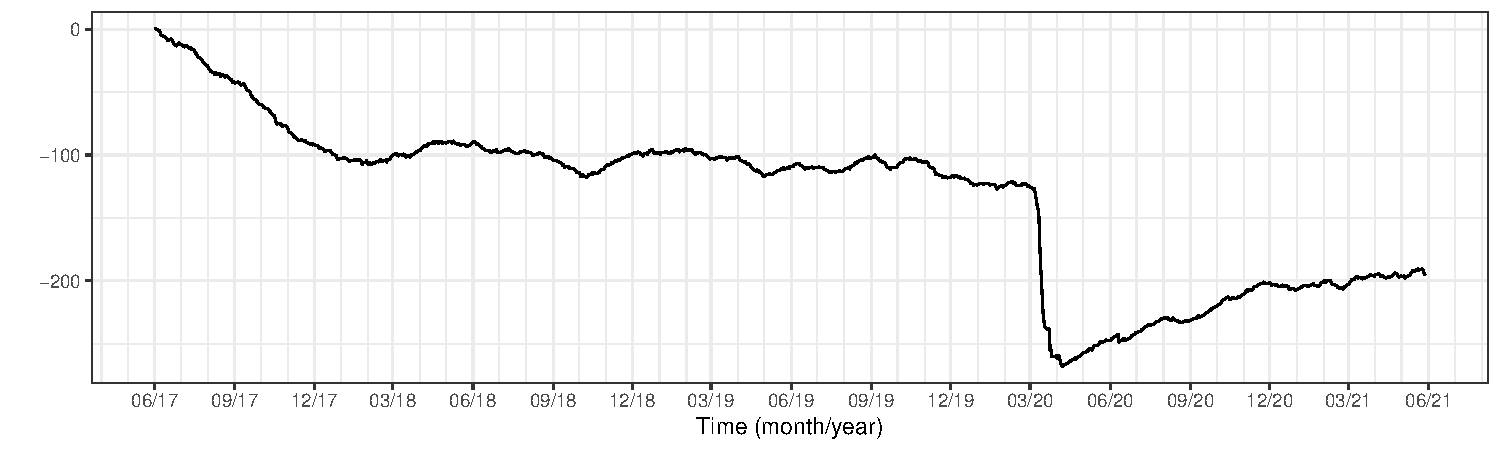
\includegraphics{new-draft_files/figure-latex/cll_plot-1} 

}

\caption{Relative log-likelihood}\label{fig:cll_plot}
\end{figure}

Overall, this analysis shows how a model with stochastic volatility is
better at describing and predicting the considered time-frame of S\&P500
returns. As can be seen from the graph and perhaps unsurprisingly, the
density forecast given the stochastic volatility model represents a
particularly significant improvement in the period of extreme values of
returns in March 2020.

\backmatter
\end{document}
